\chapter{Algoritmo de sincronización y control de formaciones}
El algoritmo de sincronización y control de formaciones funciona con dos controladores principales. El primero es el algoritmo de sincronización y control centralizado llamado ``supervisor'' y el segundo es el algoritmo de control de uniciclo para los agentes. En este capítulo se explicará el funcionamiento de cada controlador y la lógica detrás de cada uno para cumplir con las tareas de formación, evasión de colisiones y movilización hacia un objetivo.

\subsection{Controlador del supervisor}
El programa del supervisor tiene como tarea coordinar a los agentes, realizar procesamiento de datos y generar trayectorias para movilizar a los agentes hacia un objetivo evadiendo colisiones entre ellos y con los obstáculos. Para esto, el algoritmo cuenta con diferentes segmentos.

\subsubsection{Adquisición de posiciones}
La primera parte del algoritmo consiste en la toma de posiciones $X$ y $Y$ actuales de los agentes, obstáculos y el objetivo. 

\subsubsection{Cálculo de velocidades de agentes}
Luego, se realiza el cálculo de las velocidades de los agentes para moverlos hacia su posición en la formación y hacia el objetivo de interés. Este cálculo de velocidades se realiza por medio de la ecuación de consenso con un factor de peso $\omega$ que depende de las ecuaciones de tensión y de evasión de obstáculos. 

\subsubsection{Evasión de obstáculos y colisiones}
Seguido a esto, se tiene la evasión de obstáculos y colisiones que se realiza comparando la posición actual de cada agente con la posición actual de los agentes vecinos y los obstáculos.

\subsubsection{Control proporcional}
El siguiente segmento implementa el control proporcional de la Ecuación (\ref{eq:controlador_proporcional}) para movilizar a los agentes hacia un punto de interés.

\begin{equation}
	v_{n+1} = v_n + k(x_{objetivo} - x_{agente})
	\label{eq:controlador_proporcional}
\end{equation}

Donde $v$ es la velocidad del agente y $k$ es la ganancia o constante de proporcionalidad que multiplica a la distancia entre el punto de interés y la posición del agente a evaluar. Una vez se tiene la velocidad en $X$ y $Y$ de los agentes, se calcula la norma de velocidad y esta se utiliza para la toma de decisiones dentro del algoritmo.

\subsection{Controlador de los agentes}
El programa del los agentes recibe las velocidades calculadas por el supervisor. Luego, se encarga de convertirlas en velocidad lineal y angular para calcular la velocidad de cada rueda de los Pololu 3Pi+ según el modelo del uniciclo. Este programa es individual para cada agente y solo procesa los datos para si mismo.

\subsection{Funcionamiento del algoritmo}
El algoritmo consta de las siguientes etapas para su ejecución:
\begin{itemize}
	\item Etapa 0: los agentes se movilizan hacia sus posiciones iniciales para iniciar el experimento.
	\item Etapa 1: comienza el acercamiento de agentes hasta que la norma de velocidad esté por debajo de un valor seleccionado.
	\item Etapa 2: los agentes se colocan en sus posiciones de la formación hasta que el error cuadrático medio entre la formación actual y la formación deseada esté por debajo de un valor seleccionado.
	\item Etapa 3: el líder se mueve hacia el objetivo y los agentes de la formación lo siguen.
\end{itemize}

A continuación, se muestra el diagrama de flujo para los programas del supervisor y el control de los agentes.

\begin{figure}[H]
	\centering
	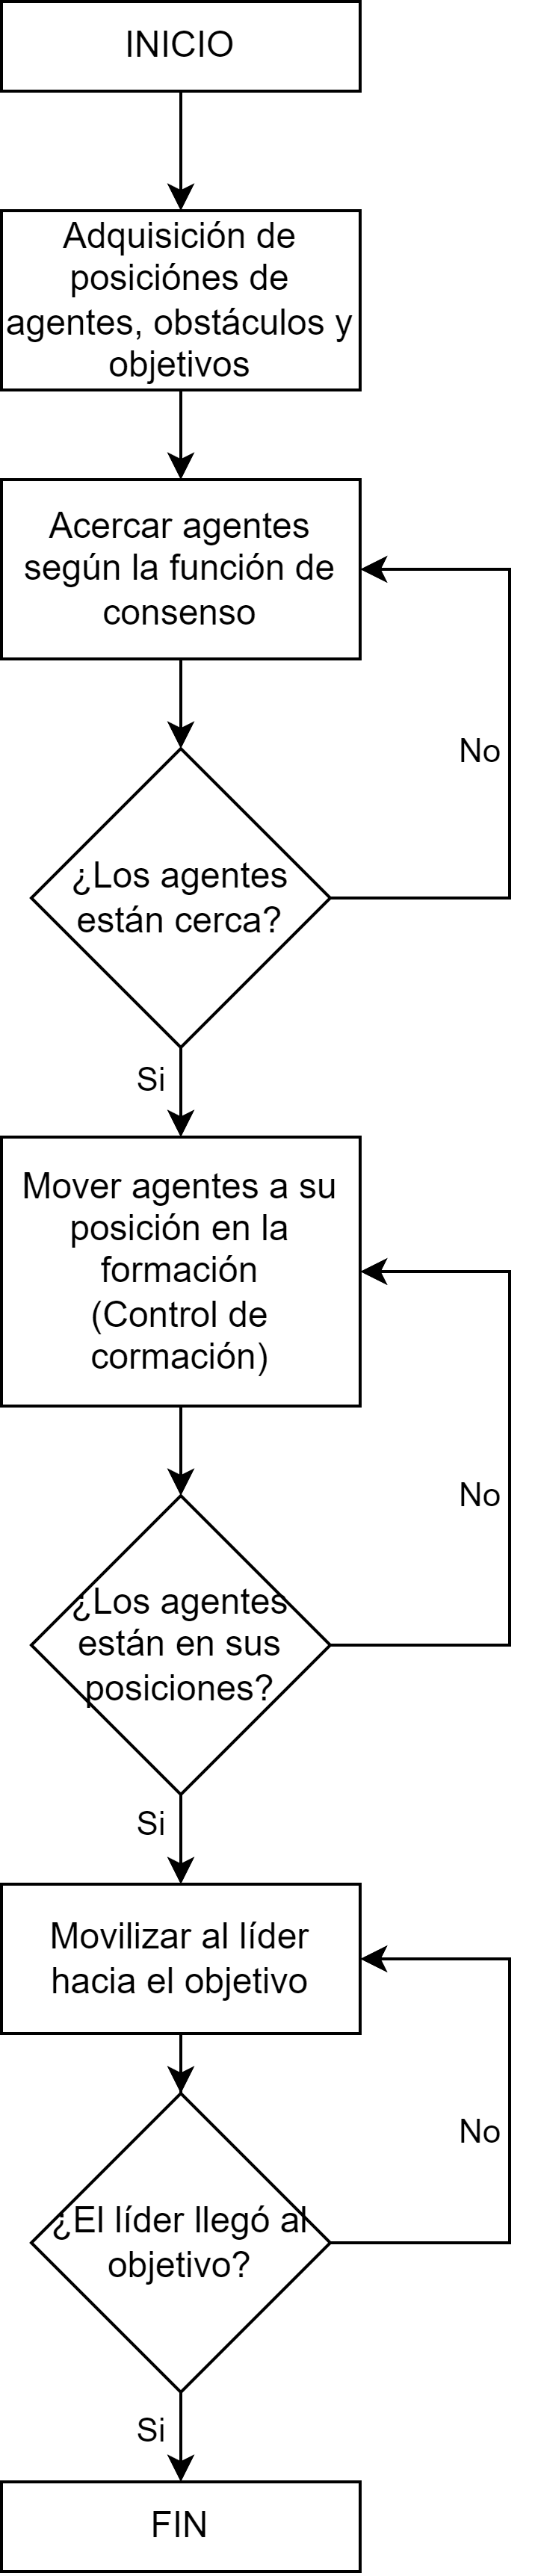
\includegraphics[width=0.2\textwidth]{diagrama_supervisor.png}
	\caption{Diagrama de flujo para el supervisor.}
	\label{fig:diagrama_supervisor}
\end{figure}

\begin{figure}[H]
	\centering
	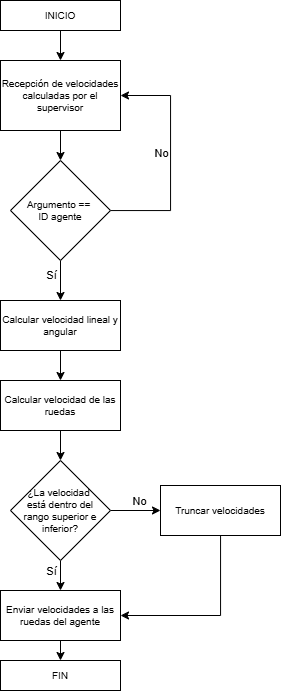
\includegraphics[width=0.35\textwidth]{diagrama_agentes.png}
	\caption{Diagrama de flujo para el programa de los agentes.}
	\label{fig:diagrama_agentes}
\end{figure}


\chapter{Restauración del algoritmo desarrollado en fases previas}
La implementación en físico del algoritmo de sincronización y control de formaciones llevada a cabo por José Alejandro Rodríguez \cite{RodriguezJA_2023_tesis} se realizó en Webots con la versión 2023b. Esta es la misma versión que la utilizada en la fase actual. También, se optó por utilizar Python 3.10 como lenguaje de programación para el controlador del supervisor y de los agentes ya que es una de las versiones más recientes de software, además que es la misma versión utilizada en la fase anterior. 

Por otro lado, en el Robotat se han realizado cambios en las conexiones con el servidor y los Pololu 3Pi+	por lo que se sería necesario un reajuste de parámetros.

En este capítulo se detallarán las modificaciones necesarias para la restauración del algoritmo y su correcta ejecución en simulaciones con Webots y en un entorno físico con el Robotat.


\section{Replicar simulaciones de Webots}

El primer paso de la restauración, fue recrear algunas simulaciones en Webots. Para esto, fue necesario instalar las siguientes librerías que no se encuentran dentro de la biblioteca estándar de Python:
\begin{itemize}
	\item Keyboard - versión 0.13.5
	\item NumPy - versión 1.23.2
\end{itemize}

Luego, se realizó la prueba del código para el controlador del supervisor y los agentes incluyendo sus respectivas funciones:
\begin{itemize}
	\item Supervisor: Supervisor\_simulacion\_y\_fisico\_v4.py
	\item Agentes: pruebaMatrizDifeomorfismo.py
	\item Funciones algoritmo: funciones.py, funVel.py
\end{itemize} 

\subsection{Comunicación entre supervisor y agentes}
Al ejecutar la primera simulación, se encontró que dos agentes permanecían inmóviles durante la primera etapa del algoritmo que consiste en mover a los agentes a sus posiciones iniciales, tal como se muestra en la Figura \ref{fig:delaygpu}.

\begin{figure}[H]
	\centering
	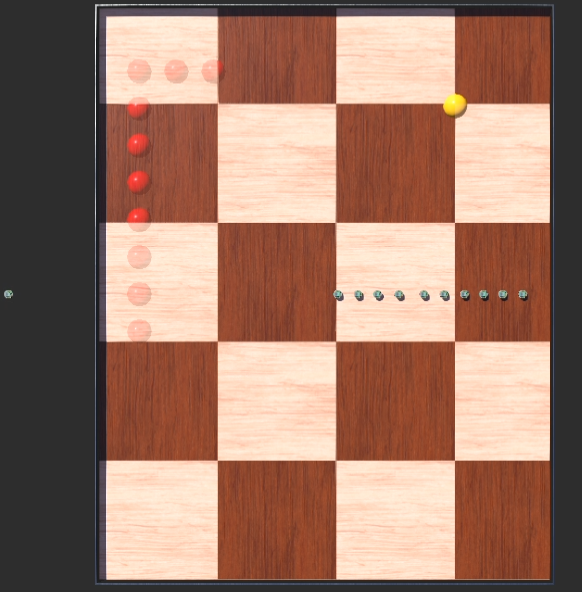
\includegraphics[width=0.30\textwidth]{delaygpu1.png}
	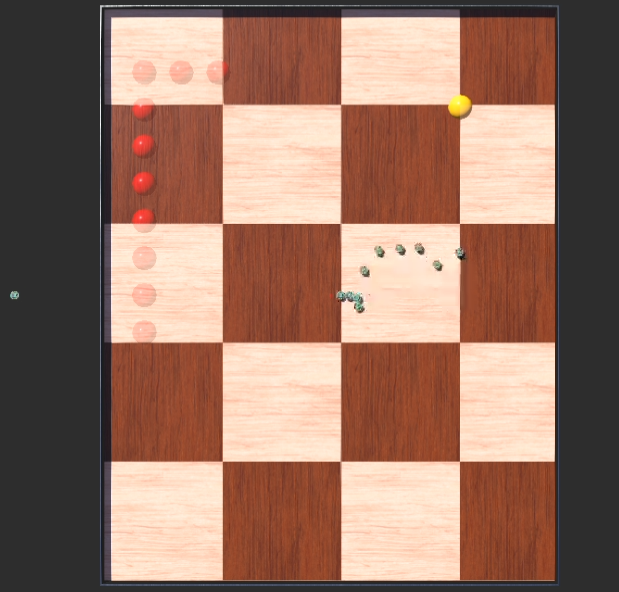
\includegraphics[width=0.30\textwidth]{delaygpu2.png}
	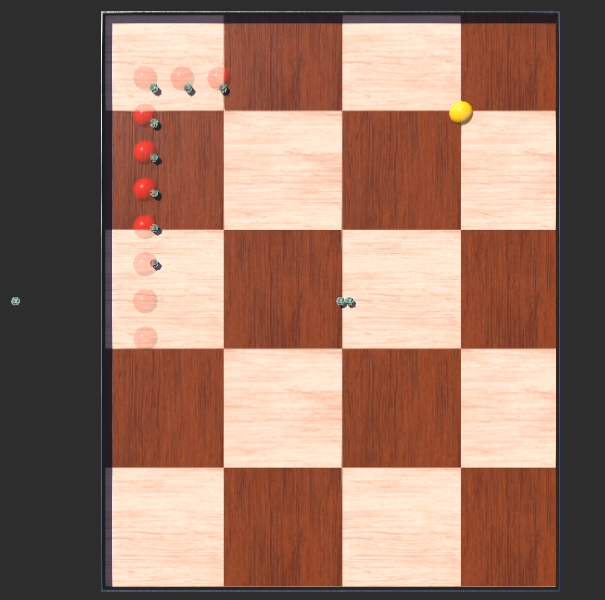
\includegraphics[width=0.30\textwidth]{delaygpu3.png}
	\caption{Ejecución de la primera simulación den Webots 2023b.}
	\label{fig:delaygpu}
\end{figure}

Esto se debe a que actualmente se está utilizando una computadora con mayor capacidad de procesamiento que la utilizada en la fase anterior. Esta capacidad de procesamiento impacta en la velocidad de ejecución de los programas. 

Dado que la comunicación entre el supervisor y los agentes se realiza por medio de una memoria compartida y la velocidad de procesamiento es mayor, el controlador de los dos primeros agentes se ejecuta antes de que el espacio de memoria compartida se haya inicializado correctamente. Para solucionar el problema, en el controlador de los agentes se agregó un tiempo de espera de 3 segundos antes de inicializar y acceder a la memoria compartida para asegurar que esta se cree correctamente en el controlador del supervisor.

\subsection{Prueba del algoritmo con simulaciones basadas en escenarios previos}
Una vez solucionado el problema de comunicación, se realizó las primeras simulaciones para replicar algunos de los escenarios realizados por José Alejandro Rodríguez \cite{RodriguezJA_2023_tesis} y comprobar el funcionamiento correcto del algoritmo. 

El código del supervisor ya cuenta con un modo de simulación en el que se ejecuta el algoritmo basado en condiciones iniciales tomadas de un escenario físico. Para esto, se debe cargar un archivo .npz que cuenta con la información necesaria para configurar la simulación según el escenario real en que se ejecutó el algoritmo.

\subsubsection{Primer escenario}
Para la primera simulación, se utilizó el archivo ``finaltrial\_6A\_AAA\_f\_1.npz'' que consiste en la siguiente configuración:
\begin{itemize}
	\item Cantidad de agentes: 6
	\item Posición inicial de agentes: línea
	\item Obstáculos: ninguno
	\item Objetivo: ubicado en la esquina
\end{itemize}

En la Figura \ref{fig:primera_simulacion}, las imágenes en el orden de izquierda a derecha y luego de arriba hacia abajo muestran la secuencia de ejecución del algoritmo.

\begin{figure}[H]
	\centering
	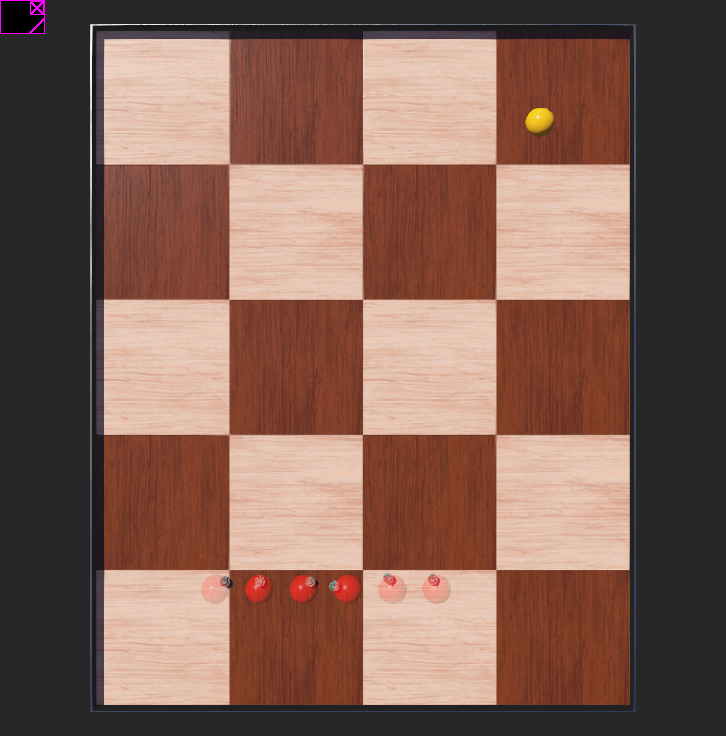
\includegraphics[width=0.45\textwidth]{sim1_p1.png}
	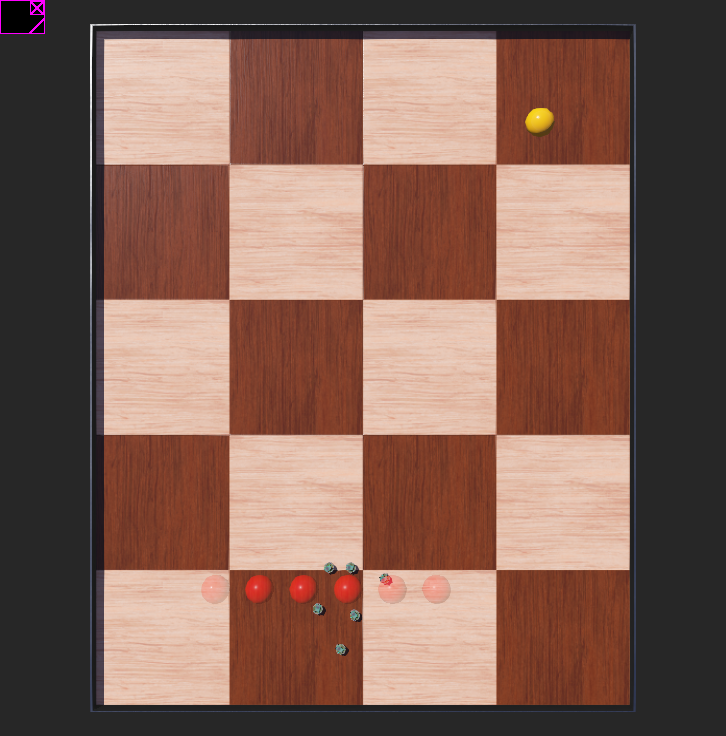
\includegraphics[width=0.45\textwidth]{sim1_p2.png}
	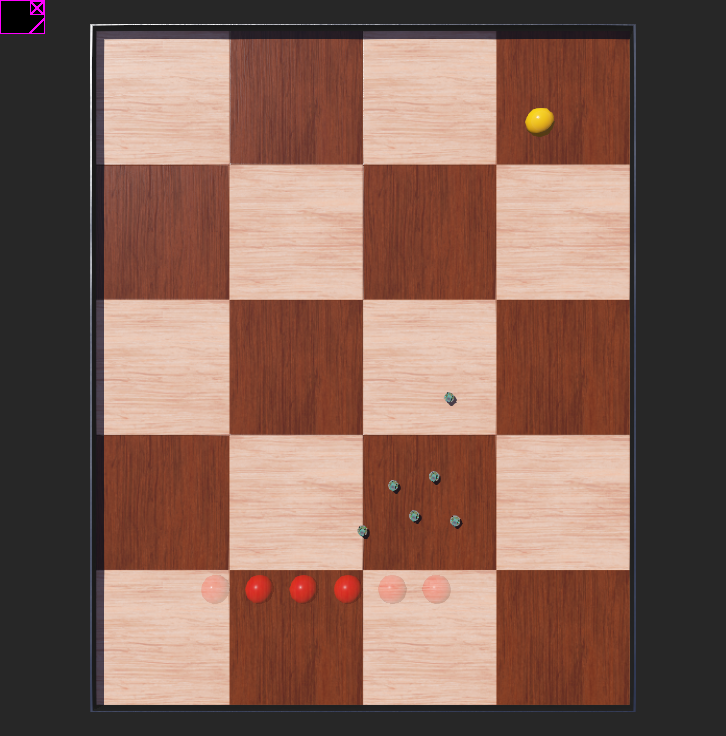
\includegraphics[width=0.45\textwidth]{sim1_p3.png}
	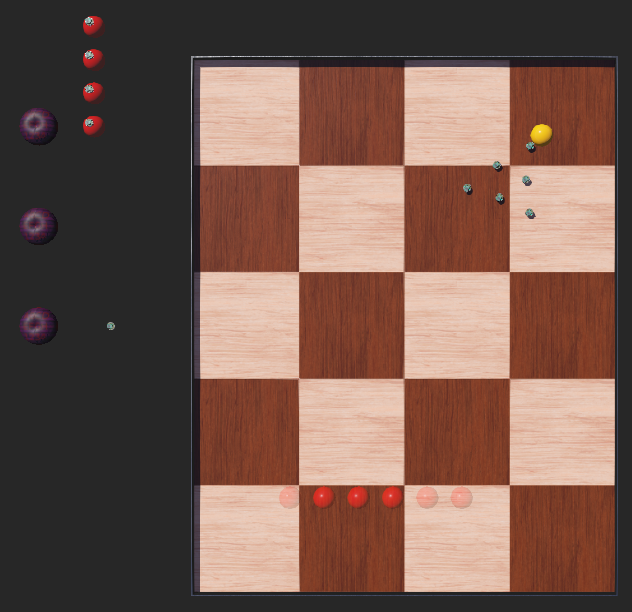
\includegraphics[width=0.45\textwidth]{sim1_p4.png}
	\caption{Ejecución del algoritmo en la primera simulación}
	\label{fig:primera_simulacion}
\end{figure}

\subsubsection{Segundo escenario}
Para la segunda simulación, se utilizó el archivo ``finaltrial\_6A\_AB1B\_f\_2.npz'' que consiste en la siguiente configuración:
\begin{itemize}
	\item Cantidad de agentes: 6
	\item Posición inicial de agentes: línea
	\item Obstáculos: ubicados en el centro
	\item Objetivo: ubicado en el centro
\end{itemize}

En la Figura \ref{fig:segunda_simulacion}, las imágenes en el orden de izquierda a derecha y luego de arriba hacia abajo muestran la secuencia de ejecución del algoritmo.

\begin{figure}[H]
	\centering
	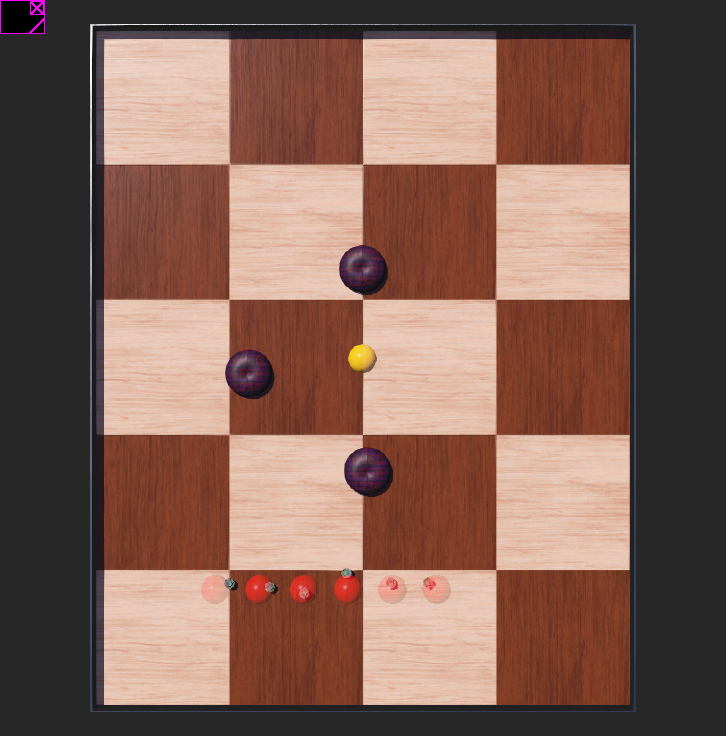
\includegraphics[width=0.45\textwidth]{sim2_p1.png}
	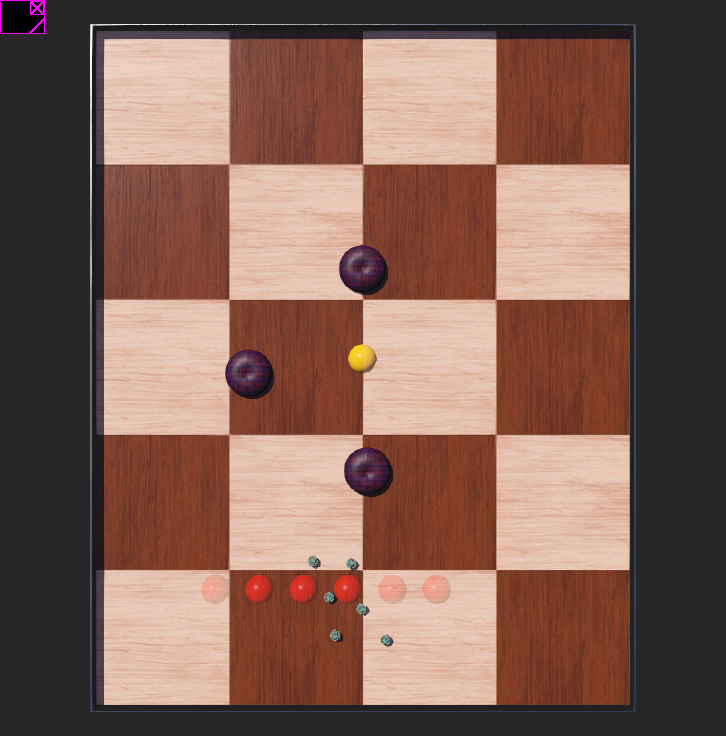
\includegraphics[width=0.45\textwidth]{sim2_p2.png}
	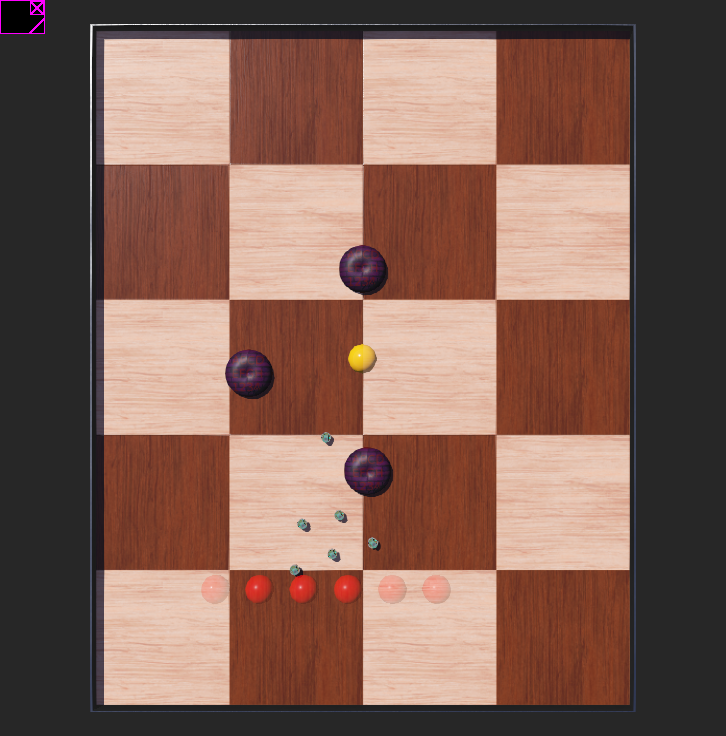
\includegraphics[width=0.45\textwidth]{sim2_p3.png}
	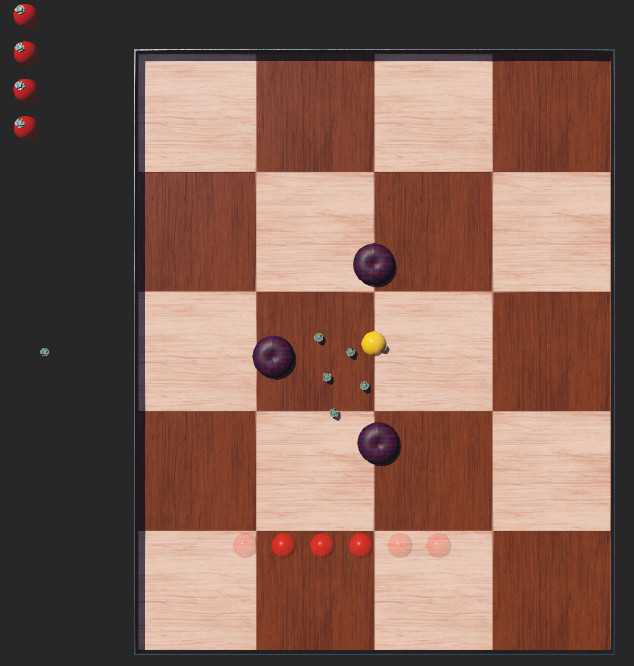
\includegraphics[width=0.45\textwidth]{sim2_p4.png}
	\caption{Ejecución del algoritmo en la segunda simulación}
	\label{fig:segunda_simulacion}
\end{figure}

\subsubsection{Tercer escenario}
Para la tercera simulación, se utilizó el archivo ``finaltrial\_6A\_BCA\_f\_1.npz'' que consiste en la siguiente configuración:
\begin{itemize}
	\item Cantidad de agentes: 6
	\item Posición inicial de agentes: círculo
	\item Obstáculos: ubicados en posiciones aleatorias
	\item Objetivo: ubicado en la esquina
\end{itemize}

En la Figura \ref{fig:tercera_simulacion}, las imágenes en el orden de izquierda a derecha y luego de arriba hacia abajo muestran la secuencia de ejecución del algoritmo.

\begin{figure}[H]
	\centering
	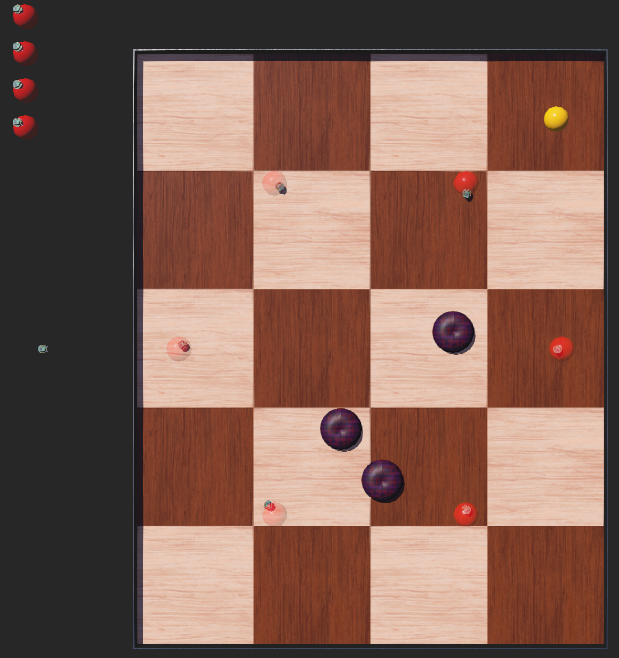
\includegraphics[width=0.45\textwidth]{sim3_p1.png}
	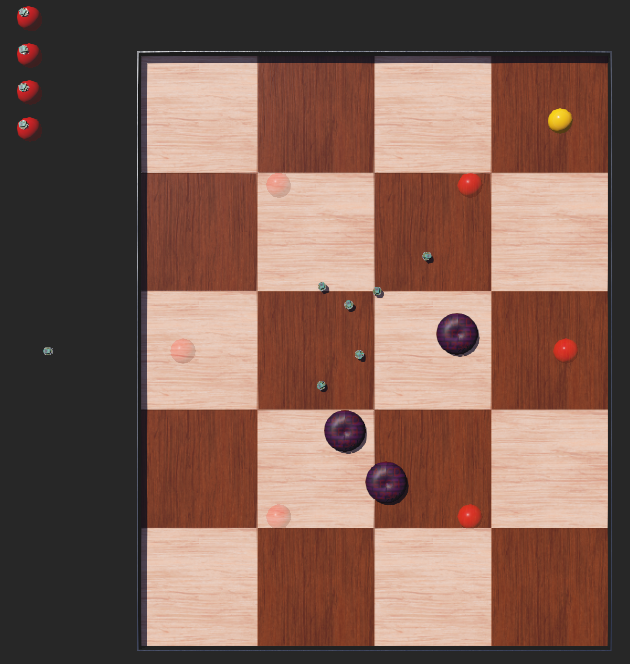
\includegraphics[width=0.45\textwidth]{sim3_p2.png}
	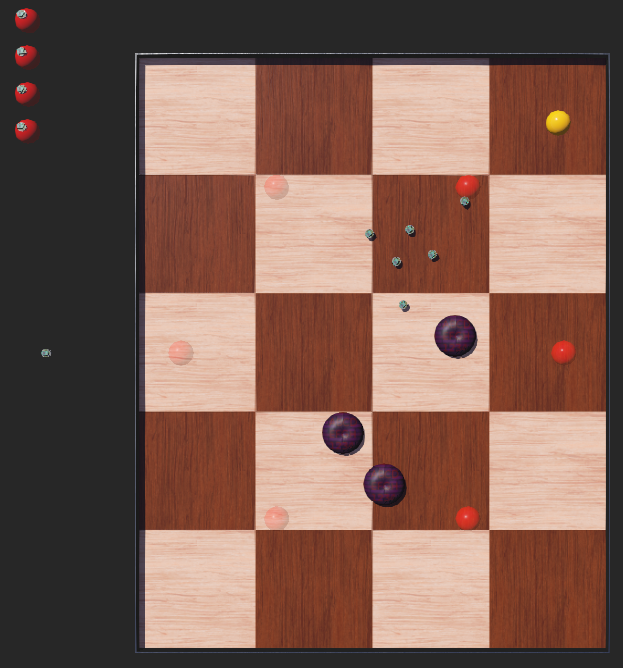
\includegraphics[width=0.45\textwidth]{sim3_p3.png}
	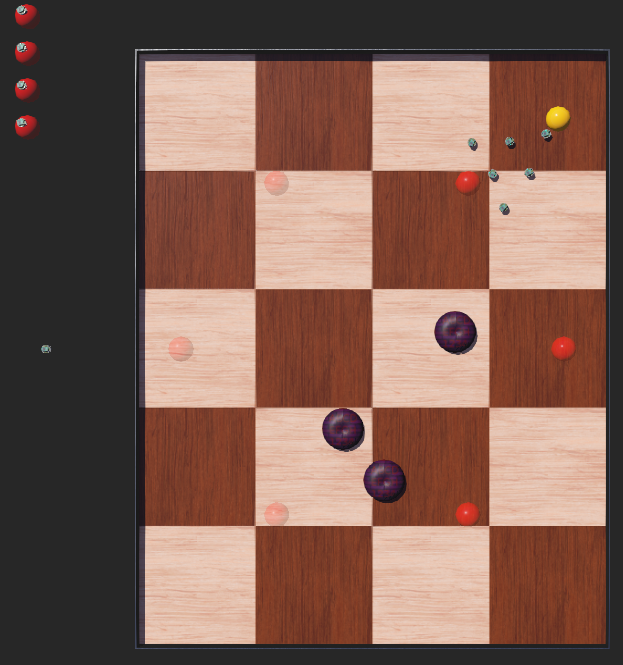
\includegraphics[width=0.45\textwidth]{sim3_p4.png}
	\caption{Ejecución del algoritmo en la tercera simulación}
	\label{fig:tercera_simulacion}
\end{figure}


%\subsection{Cambios en el entorno de simulación}
%En Webots 
%	Se cambió las medidas de la cuadrícula y de la arena para que coincida con las medidas reales

\section{Replicar el funcionamiento del algoritmo en el Robotat}
Una vez teniendo el algoritmo funcionando en Webots, el siguiente paso fue verificar que el algoritmo se ejecute correctamente en el Robotat.
\subsection{Pruebas de conexión con el Pololu 3Pi+ y el Robotat}
 Primero, se realizaron pruebas de conexión y obtención de datos con el Robotat y los Pololu 3Pi+ utilizando las funciones creadas en Python por José Alejandro Rodríguez \cite{RodriguezJA_2023_tesis}:
\begin{itemize}
	\item robotat\_connect
	\item robotat\_disconnect
	\item robotat\_get\_pose
	\item robotat\_3pi\_connect
	\item robotat\_3pi\_disconnect
	\item robotat\_3pi\_set\_wheel\_velocities
	\item robotat\_3pi\_force\_stop
\end{itemize}

Al realizar las pruebas de conexión con los agentes Pololu 3Pi+ se tenía el error mostrado en la Figura \ref{fig:error_conexion}. Este error se debe a que hubo un cambio en los puertos de conexión con el ESP$32$ de los agentes. Anteriormente la conexión se realizaba en el puerto $8888$ y actualmente se realiza en el puerto $9090$. Al actualizar este dato dentro de la función ``robotat\_3pi\_connect''  en del archivo ``funciones\_conjunto\_3pi.py'' se logró una conexión exitosa con el agente para el envío de comandos de velocidades.

\begin{figure}[H]
	\centering
	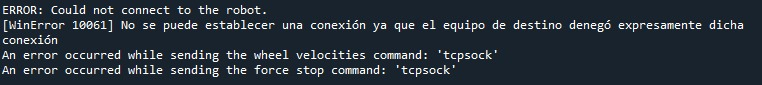
\includegraphics[width=0.8\textwidth]{error_conexion.png}
	\caption{Error de conexión con Pololu 3Pi+.}
	\label{fig:error_conexion}
\end{figure}

\subsection{Calibración de marcadores}
Una vez lograda la conexión con los Pololu 3Pi+, se tuvo que realizar una nueva calibración de los marcadores del OptiTrack para obtener el desfase del ángulo orientación (\textit{bearing}) de cada marcador. Estos desfases son diferentes en cada marcador y se producen por la forma en que el OptiTrack identifica cada uno según la posición de sus esferas reflectivas.

En la fase anterior, se realizó una calibración con los marcadores del $1$ al $15$, sin embargo, se agregaron nuevos marcadores por lo que ahora se cuenta con $22$ de ellos para utilizar, de los cuales están inhabilitados el $1$ y $9$ ya que serán utilizados en otros proyectos de graduación. Por tanto, ahora se tienen disponibles los marcadores de la Figura \ref{fig:marcadores_disponibles}. 

Para corregir el desfase de cada marcador, primero se obtiene la orientación con ángulos de Euler en la secuencia $zyx$, luego, al primer ángulo que representa la rotación respecto al eje $z$ se le resta el desfase obtenido $\theta_z$. Para realizar la calibración, se colocaron todos los marcadores disponibles de la Figura \ref{fig:marcadores_disponibles} con la misma orientación sobre el eje $y$ de la mesa de pruebas del Robotat tal como se observa en la Figura \ref{fig:marcadores_calibracion}.

\begin{figure}[H]
	\centering
	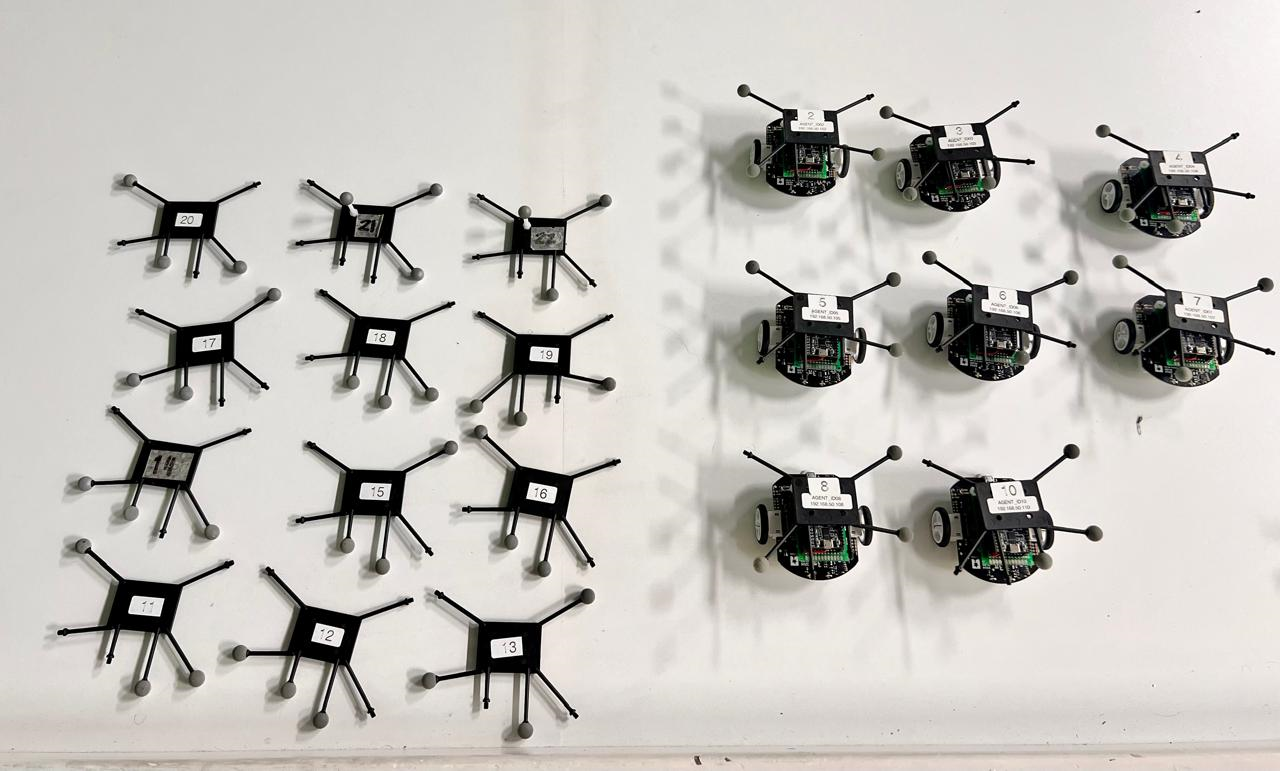
\includegraphics[width=0.8\textwidth]{marcadores_disponibles.png}
	\caption{Marcadores del OptiTrack disponibles para su uso.}
	\label{fig:marcadores_disponibles}
\end{figure}

\begin{figure}[H]
	\centering
	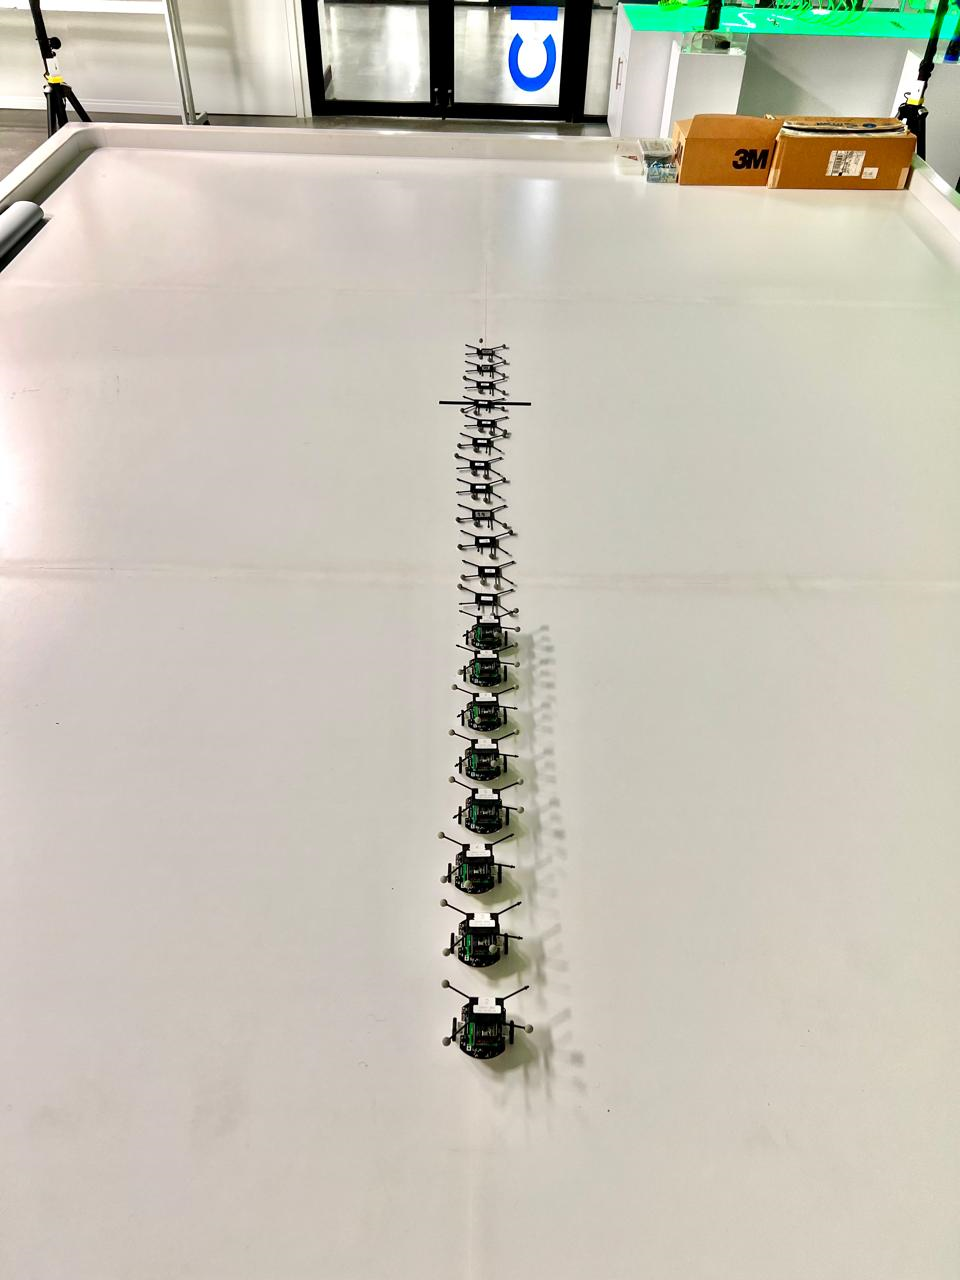
\includegraphics[width=0.6\textwidth]{marcadores_ejey.png}
	\caption{Marcadores alineados sobre el eje $y$ de la mesa de pruebas del Robotat.}
	\label{fig:marcadores_calibracion}
\end{figure}

Al obtener la pose de cada marcador, se realizó la conversión a ángulos de Euler en la secuencia $zyx$ y se obtuvo los ángulos de desfase del Cuadro \ref{cuadro:desfases_iniciales}. Al comparar los desfases actuales con los obtenidos en la fase previa mostrados en el Cuadro \ref{cuadro:desfases_anteriores}, se observó que los valores son similares por lo que se optó tomar los desfases anteriores para los marcadores $1$ y $9$ faltantes en la calibración actual. Por último, en el Cuadro \ref{cuadro:desfases_finales} se observan los desfases finales para cada uno de los marcadores del $1$ al $22$. Estos valores se guardaron en un archivo .npy llamado ``nueva\_calibracion\_markers\_1\_al\_22.npy'' para aplicarlos luego de obtener la pose de cada marcador en el algoritmo y así tener siempre un ángulo respecto del eje $z$ igual a cero ($\theta_z$ = 0).

\begin{table}[H]
	\centering
	\begin{tabular}{|l|l|}
		\hline
		\textbf{Marcador} & \textbf{Desfase  $\theta_z$ en grados} \\ \hline
		2 & -47.2746822 \\ \hline
		3 & -90.32278167 \\ \hline
		4 & -135.7890952 \\ \hline
		5 & 179.3715195 \\ \hline
		6 & -141.0274548 \\ \hline
		7 & -175.0541793 \\ \hline
		8 & -78.11543097 \\ \hline
		10 & 143.2079276 \\ \hline
		11 & 111.0832797 \\ \hline
		12 & 166.1718189 \\ \hline
		13 & -127.3111755 \\ \hline
		14 & -109.4993486 \\ \hline
		15 & -40.73944282 \\ \hline
		16 & -104.1691129 \\ \hline
		17 & -121.1927571 \\ \hline
		18 & -92.48122033 \\ \hline
		19 & 4.298050244 \\ \hline
		20 & -133.2161012 \\ \hline
		21 & -112.0477043 \\ \hline
		22 & -15.28469666 \\ \hline
	\end{tabular}
	\caption{Desfases de marcadores disponibles alineados con el eye $y$ de la mesa de pruebas del Robotat.}
	\label{cuadro:desfases_iniciales}
\end{table}

\begin{table}[H]
	\centering
	\begin{tabular}{|l|l|}
		\hline
		\textbf{Marcador} & \textbf{Desfase $\theta _{z}$ en grados} \\ \hline
		1                 & 91.99470274710572                      \\ \hline
		2                 & -46.814569482191594                    \\ \hline
		3                 & -92.39049071644509                     \\ \hline
		4                 & -138.20668559103328                    \\ \hline
		5                 & 176.37515477240987                     \\ \hline
		6                 & -144.1821533175259                     \\ \hline
		7                 & -176.31925348204803                    \\ \hline
		8                 & -79.95245389000435                     \\ \hline
		9                 & -9.87621045801094                      \\ \hline
		10                & 139.3578557303511                      \\ \hline
		11                & 111.93284607034238                     \\ \hline
		12                & 167.57610128913143                     \\ \hline
		13                & -128.0708601137765                     \\ \hline
		14                & -111.1403638963379                     \\ \hline
		15                & -43.41121657780576                     \\ \hline
	\end{tabular}
	\caption{Desfases de marcadores obtenidos en la fase previa por José Alejandro Rodríguez \cite{RodriguezJA_2023_tesis}.}
	\label{cuadro:desfases_anteriores}
\end{table}

\begin{table}[!ht]
	\centering
	\begin{tabular}{|l|l|}
		\hline
		\textbf{Marcador} & \textbf{Desfase $\theta_z$ en grados} \\ \hline
		1 & 91.99470275 \\ \hline
		2 & -47.2746822 \\ \hline
		3 & -90.32278167 \\ \hline
		4 & -135.7890952 \\ \hline
		5 & 179.3715195 \\ \hline
		6 & -141.0274548 \\ \hline
		7 & -175.0541793 \\ \hline
		8 & -78.11543097 \\ \hline
		9 & -9.876210458 \\ \hline
		10 & 143.2079276 \\ \hline
		11 & 111.0832797 \\ \hline
		12 & 166.1718189 \\ \hline
		13 & -127.3111755 \\ \hline
		14 & -109.4993486 \\ \hline
		15 & -40.73944282 \\ \hline
		16 & -104.1691129 \\ \hline
		17 & -121.1927571 \\ \hline
		18 & -92.48122033 \\ \hline
		19 & 4.298050244 \\ \hline
		20 & -133.2161012 \\ \hline
		21 & -112.0477043 \\ \hline
		22 & -15.28469666 \\ \hline
	\end{tabular}
	\caption{Desfases finales para calibración de marcadores del $1$ al $22$.}
	\label{cuadro:desfases_finales}
\end{table}

\subsection{Selección de marcadores a utilizar}
Una vez guardada la calibración de marcadores, se realizó pruebas en el Robotat para ejecutar el algoritmo de sincronización y control de formaciones. Sin embargo, el primer problema que se identificó fue que al menos un agente siempre permanecía inmóvil. En la Figura \ref{fig:agente_inmovil} se observa la ejecución del algoritmo donde únicamente se mueve un agente de los dos utilizados.

\begin{figure}[H]
	\centering
	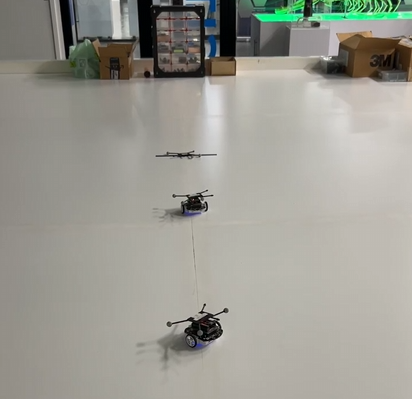
\includegraphics[width=0.6\textwidth]{agente_inmovil_p1.png}
	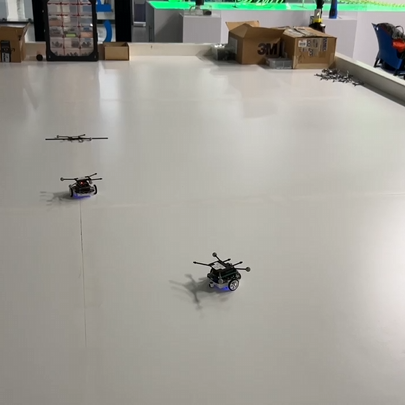
\includegraphics[width=0.6\textwidth]{agente_inmovil_p2.png}
	\caption{Problema de funcionamiento en físico, agentes permanecen inmóviles.}
	\label{fig:agente_inmovil}
\end{figure}

Anteriormente, para obtener las poses de los marcadores se utilizaba una lista predeterminada con los valores enteros del $1$ al $12$ en orden ascendente que serían los marcadores a utilizar. Sin embargo esto ocasionaba diferentes problemas.

Para obtener las poses de los marcadores se utiliza la función ``robotat\_get\_pose'', esta recibe como argumentos el objeto TCP y los números de marcadores. Al tener una lista predeterminada de valores, siempre se está solicitando la pose de los $12$ marcadores aunque no todos estén en uso, resultando en una solicitud de datos innecesaria para el servidor. Además, dado que actualmente no se tienen disponibles los marcadores $1$ y $9$, se excede el tiempo de espera (\textit{Time Out}) para obtención de la pose de estos, lo que resulta en tiempos muertos durante la ejecución del código.

Para solucionar el problema, se optó por solicitar únicamente las poses de los marcadores a utilizar con una lista que contiene los números de todos los marcadores con el orden: agentes, objetivo y obstáculos. A continuación se muestra un ejemplo de esto.

Marcadores de agentes $= [1, 2, 3, 4]$

Marcador del objetivo $ = [22]$

Marcadores de obstáculos = $ = [14, 15, 16]$

Marcadores a solicitar $ = [1, 2, 3, 4, 22, 14, 15, 16]$


Por otro lado, para asignar los marcadores de cada agente, se debía elegir un intervalo  de valores consecutivos de manera ascendente dentro de la lista predeterminada. Esto era problemático ya que limita a utilizar únicamente los agentes dentro del intervalo seleccionado, por lo que si un agente se descargaba, era obligatorio reemplazar las baterías para volver a utilizarlo. Por esto, se optó por cambiar la asignación de los marcadores para cada agente permitiendo seleccionar cualquier marcador disponible en el Robotat sin algún orden específico y ahora, para obtener las poses de los marcadores, únicamente se solicitan los datos al servidor de los marcadores en uso. Esto además, permite agilizar las pruebas a realizar ya que en múltiples ocasiones es necesario compartir los agentes Pololu 3Pi+ con otros compañeros.

En la Figura \ref{fig:seleccion_agentes}, el número dentro del círculo, representa el número de marcador asignado al agente. A la izquierda se puede observar la asignación de los marcadores a cada agente con la implementación del algoritmo original, mientras del lado derecho se observa una asignación arbitraria luego del cambio mencionado.


\begin{figure}[H]
	\centering
	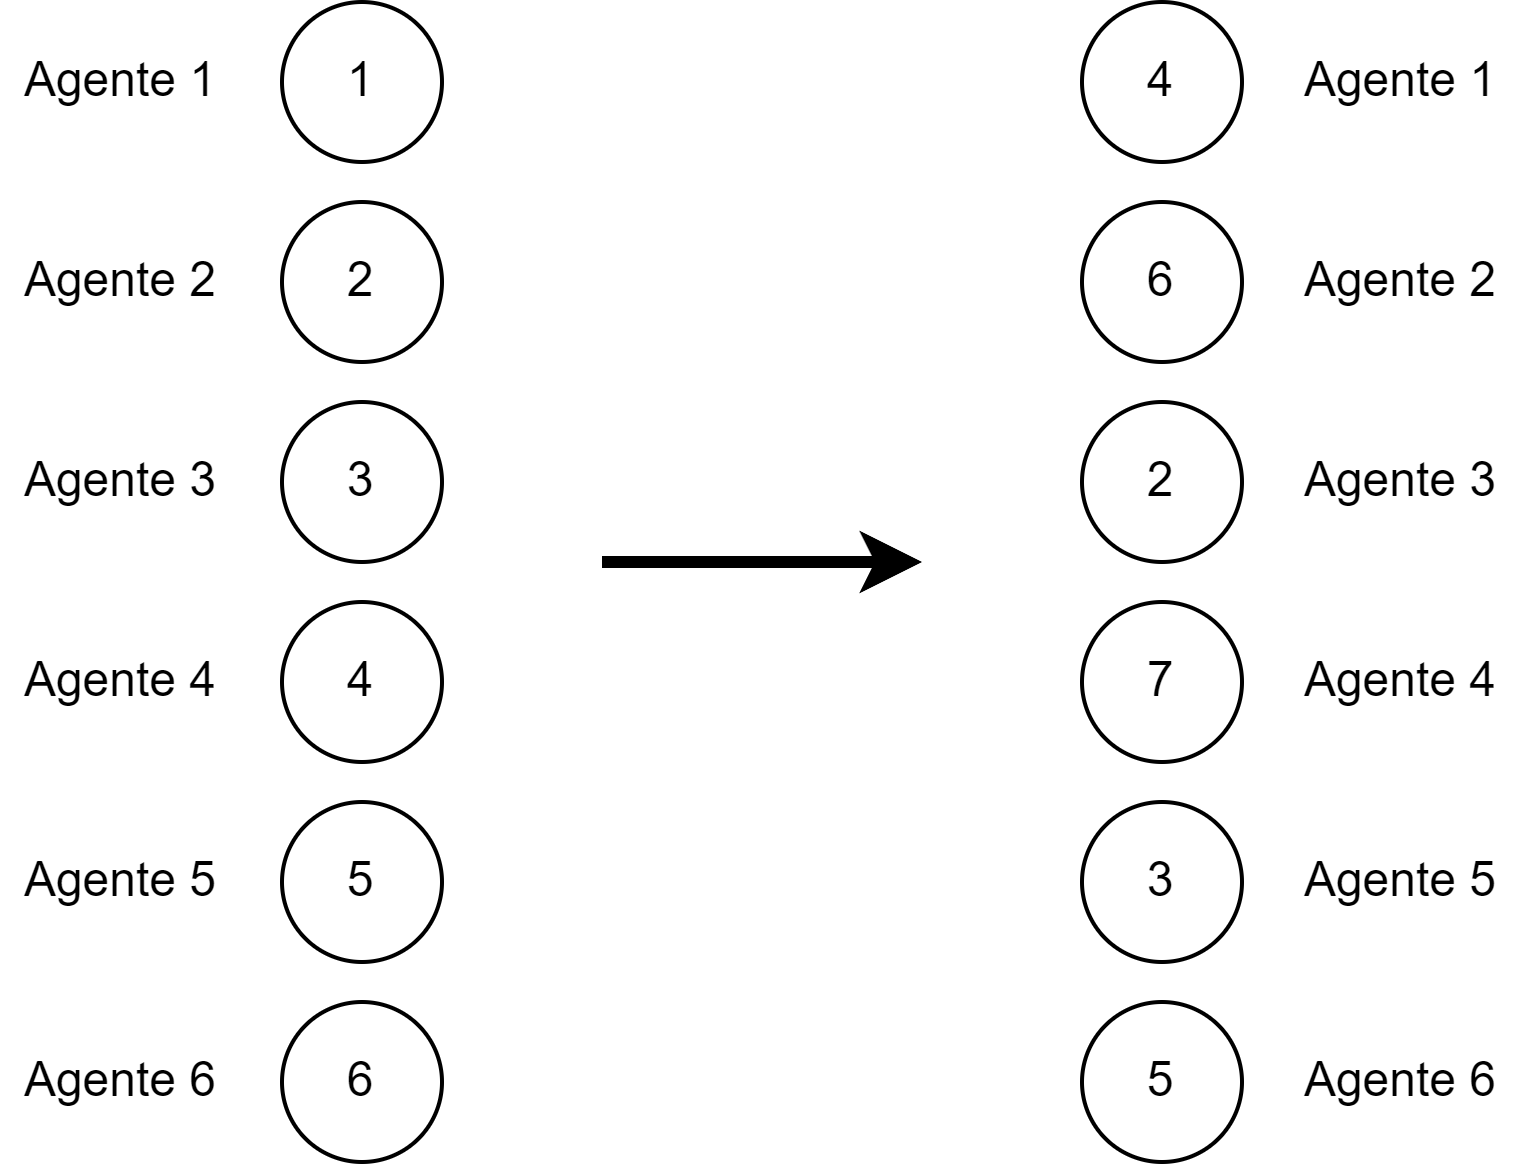
\includegraphics[width=0.6\textwidth]{seleccion_agentes.png}
	\caption{Selección de marcadores para cada agente antes y después de las modificaciones.}
	\label{fig:seleccion_agentes}
\end{figure}


\subsection{Ajuste de parámetros en el algoritmo}
Una vez realizadas las modificaciones anteriores, al ejecutar el algoritmo en físico con tres agentes se encontró que su comportamiento es divergente en la etapa donde se movilizan hacia sus posiciones iniciales. En la Figura \ref{fig:divergencia1} se observa la trayectoria que toman los agentes.

\begin{figure}[H]
	\centering
	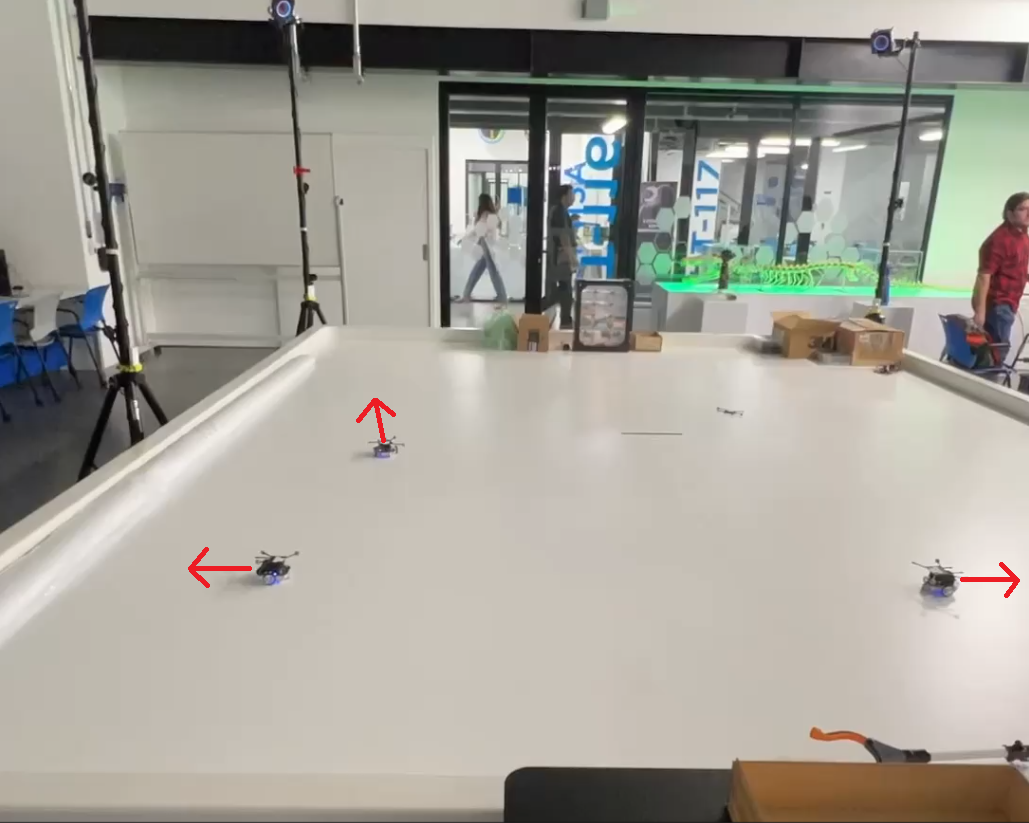
\includegraphics[width=0.6\textwidth]{divergencia_p1.png}
	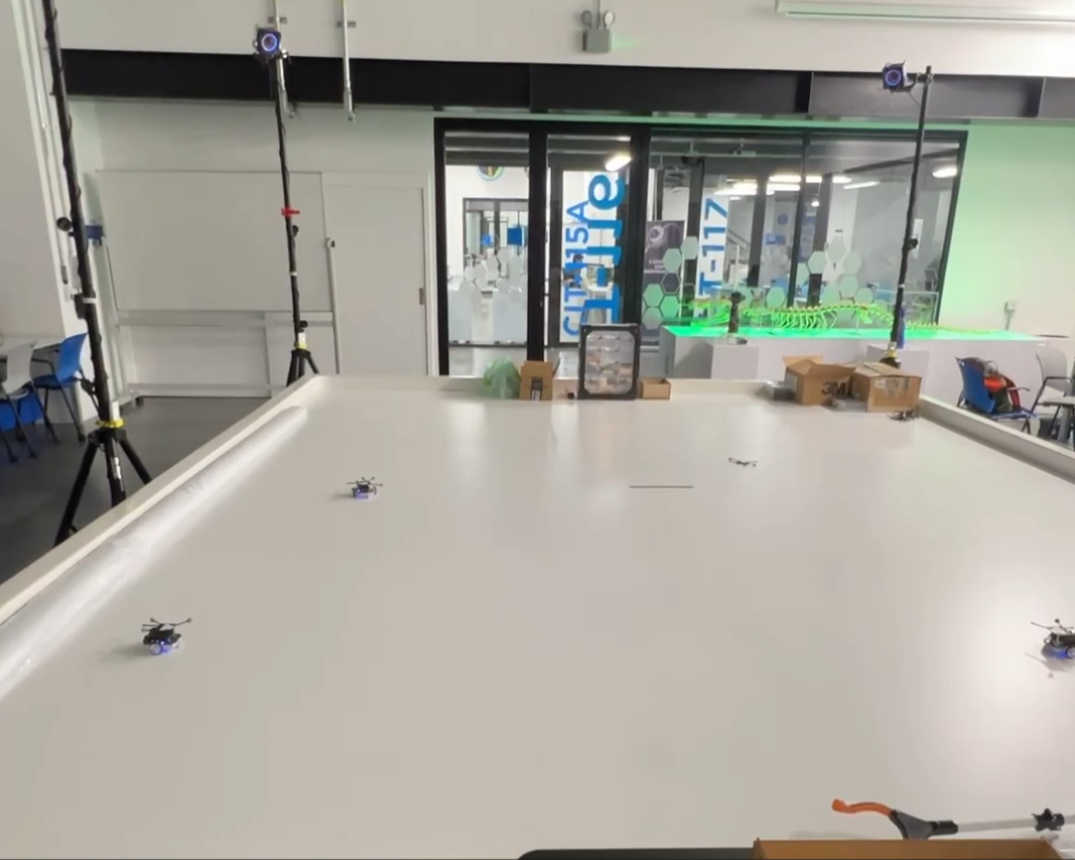
\includegraphics[width=0.6\textwidth]{divergencia_p2.png}
	\caption{Problema de funcionamiento en físico, agentes divergen hacia posiciones iniciales. }
	\label{fig:divergencia1}
\end{figure}

Para intentar solucionar esto, se invirtió signo de la constante de proporcionalidad en el control de velocidad aplicado en la etapa 0 del algoritmo. Anteriormente se utilizaba $k = 5$, ahora se utiliza $k = -5$. Al aplicar el cambio, se encontró que ahora los agentes si se colocan en sus posiciones iniciales, sin embargo, ahora el comportamiento de divergencia se sigue presentando en las demás etapas del algoritmo tal como se observa en la Figura \ref{fig:divergencia2}.

\begin{figure}[H]
	\centering
	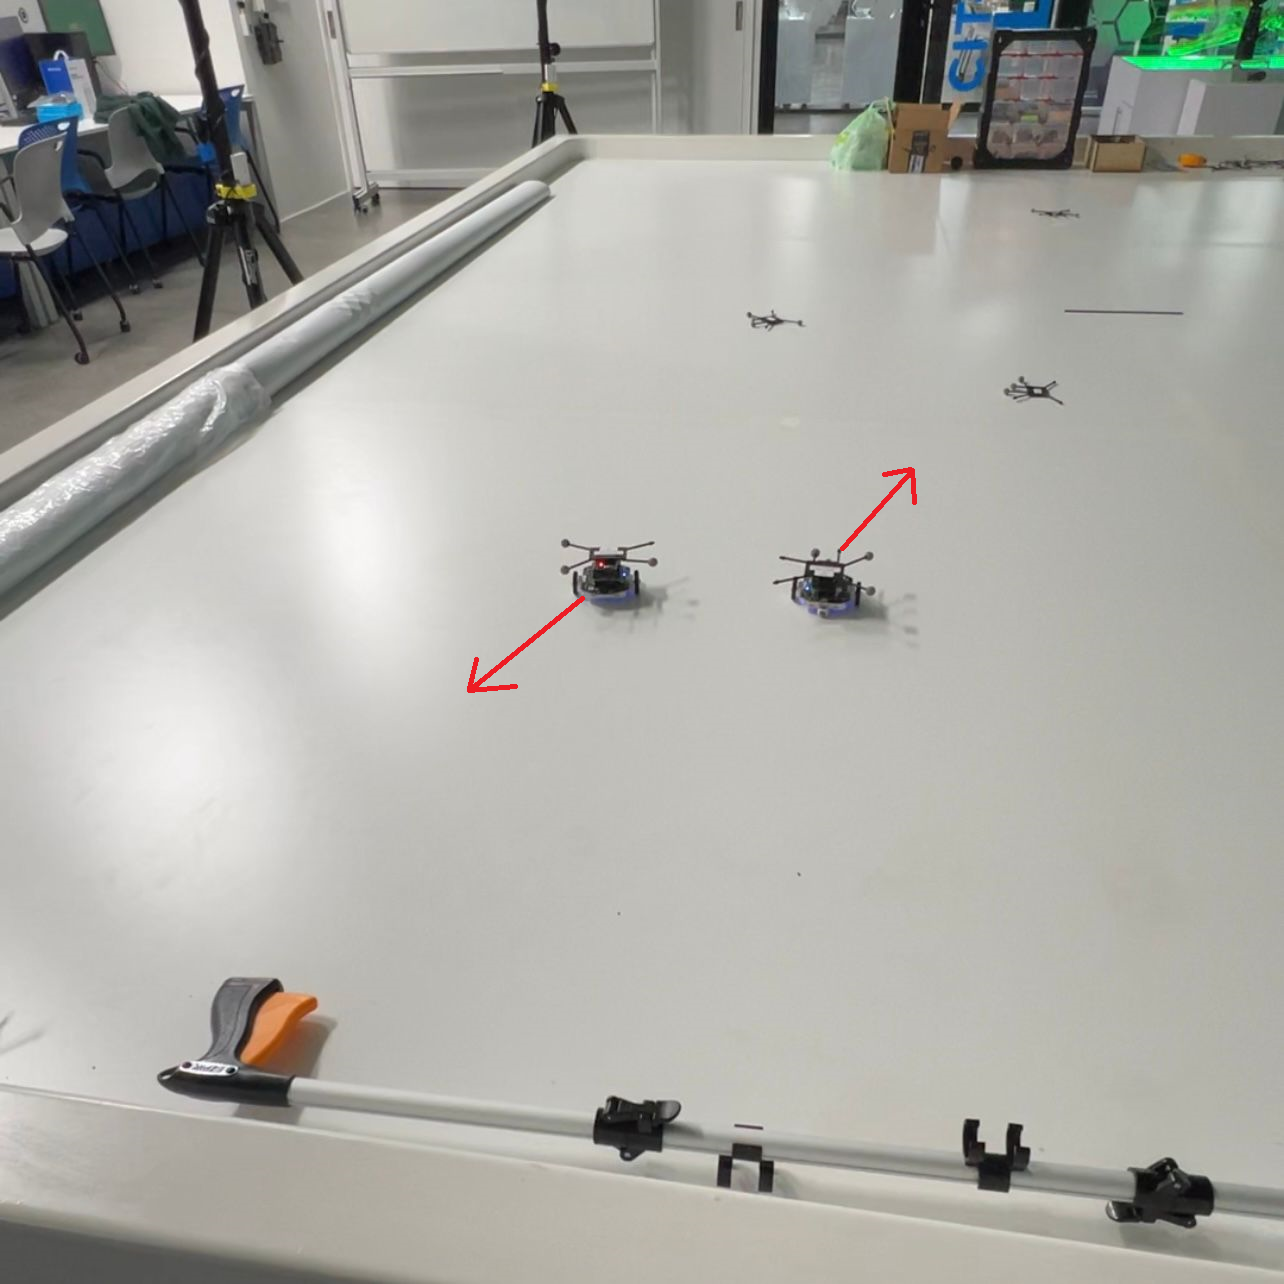
\includegraphics[width=0.6\textwidth]{divergencia2_p1.png}
	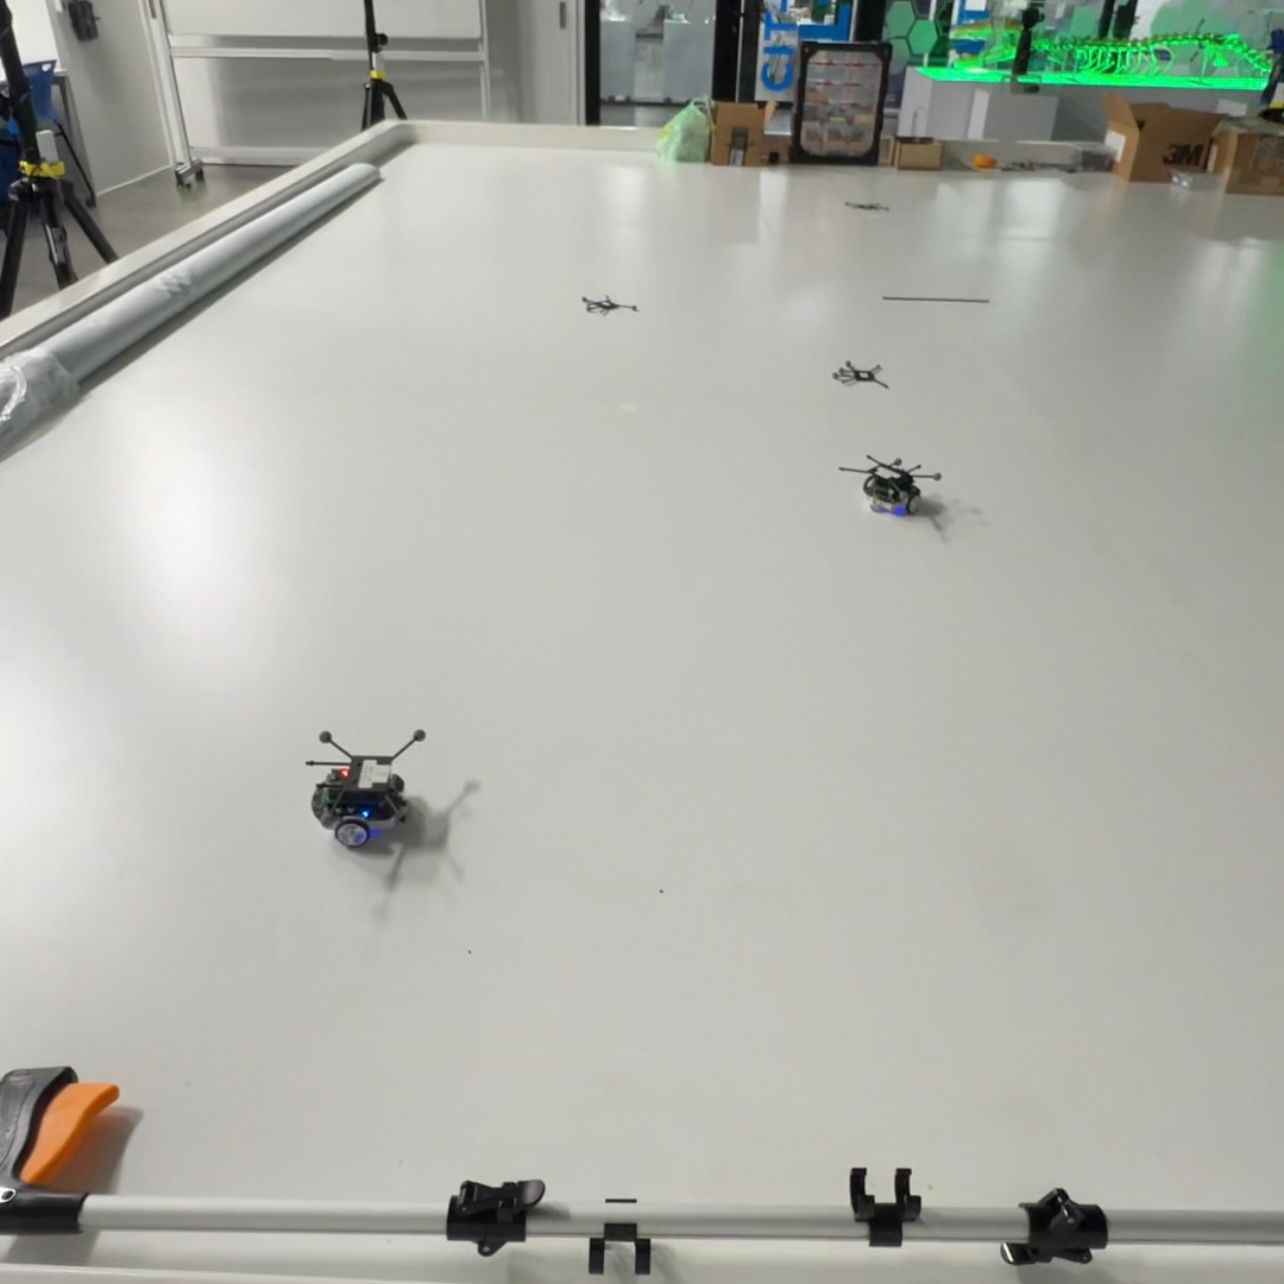
\includegraphics[width=0.6\textwidth]{divergencia2_p2.png}
	\caption{Problema de funcionamiento en físico, agentes divergen luego de colocarse en sus posiciones iniciales.}
	\label{fig:divergencia2}
\end{figure}

Al observar esto, se encontró que el patrón de divergencia se presentaba en todas las secciones donde se aplica el control proporcional para la velocidad de los agentes. Sabiendo esto, se optó por invertir el signo de la velocidad $v_n$ y la constante $k$ de la Ecuación (\ref{eq:controlador_proporcional}) tal como se observa a continuación:

\begin{equation}
	v_{n+1} = -v_n - k(x_{objetivo} - x_{agente})
	\label{eq:controlador_proporcional2}
\end{equation}

Con esto, se logró solucionar la divergencia de los agentes y se realizó la primera ejecución del algoritmo exitosa utilizando dos agentes, sin obstáculos tal como se observa en la Figura \ref{fig:prueba_fisico1}. Las imágenes en el orden de izquierda a derecha y luego de arriba hacia abajo muestran la secuencia de ejecución del algoritmo.

\begin{figure}[H]
	\centering
	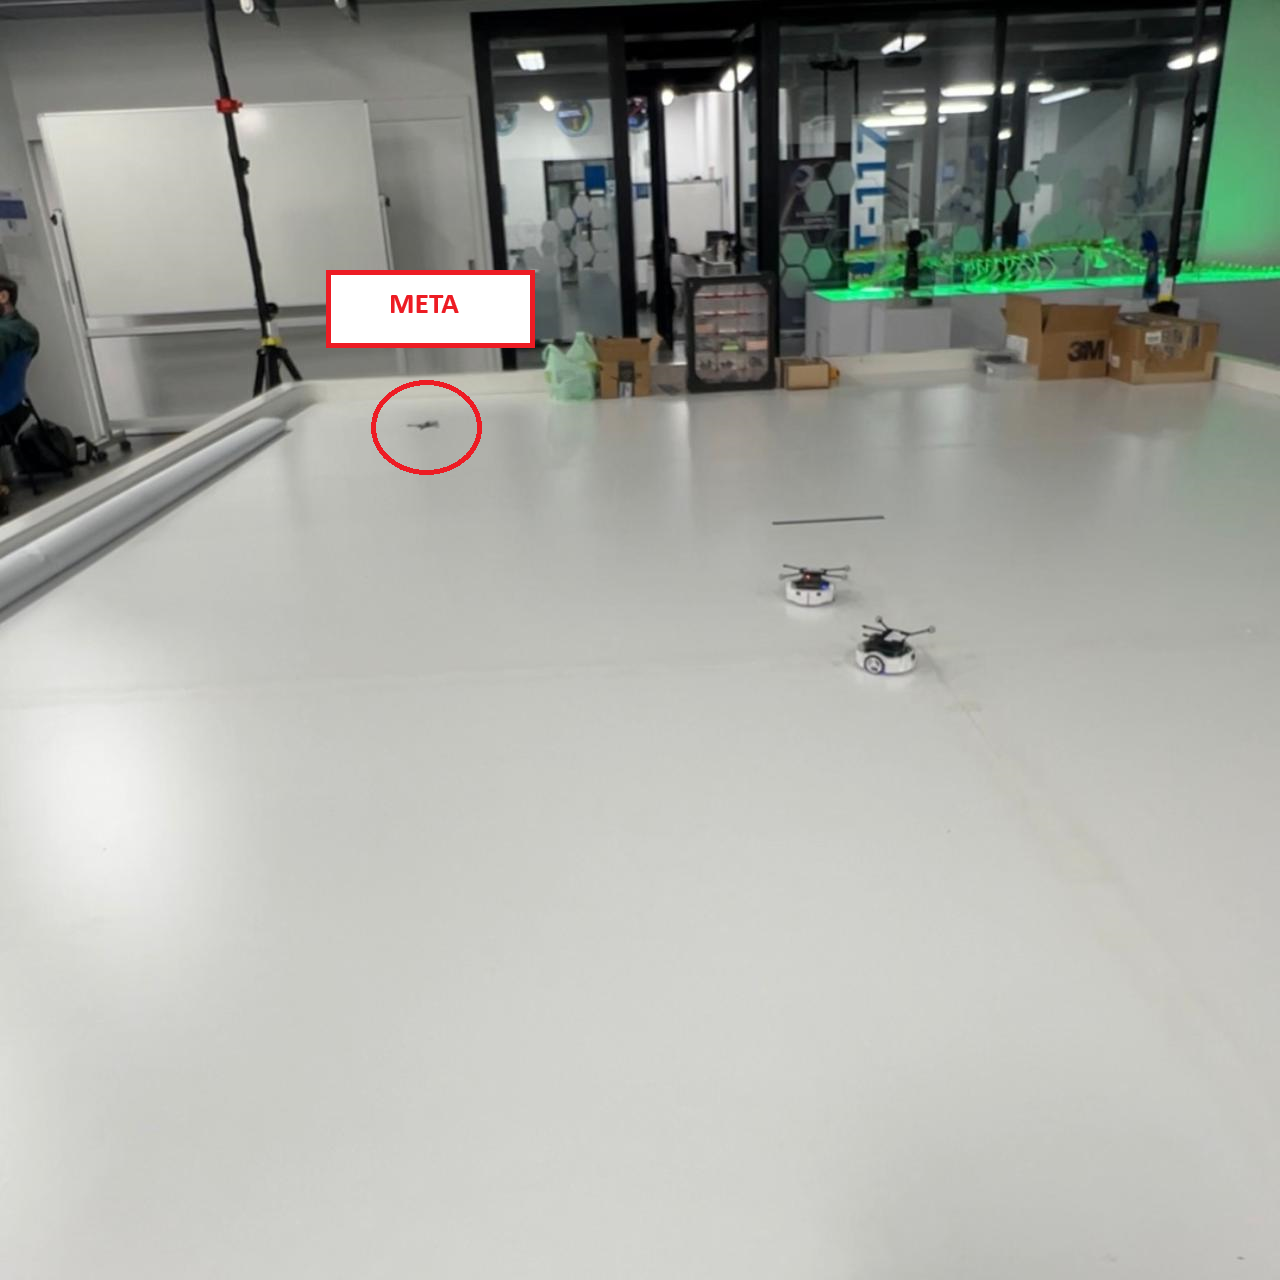
\includegraphics[width=0.45\textwidth]{prueba_fisico_p1.png}
	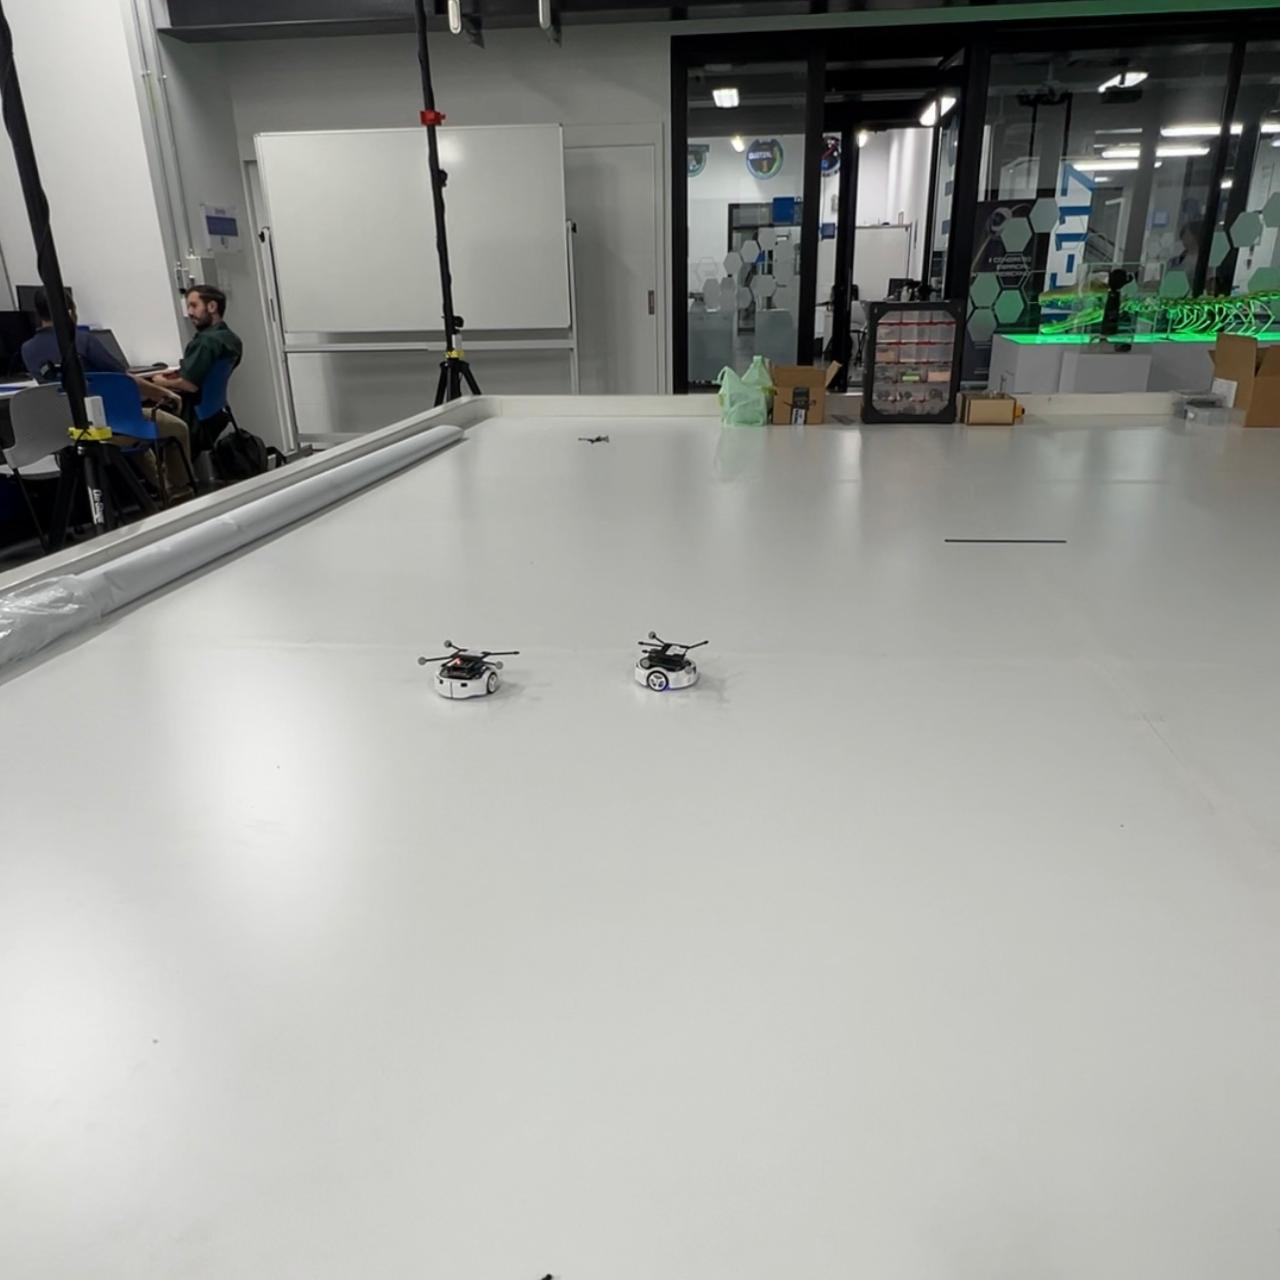
\includegraphics[width=0.45\textwidth]{prueba_fisico_p2.png}
	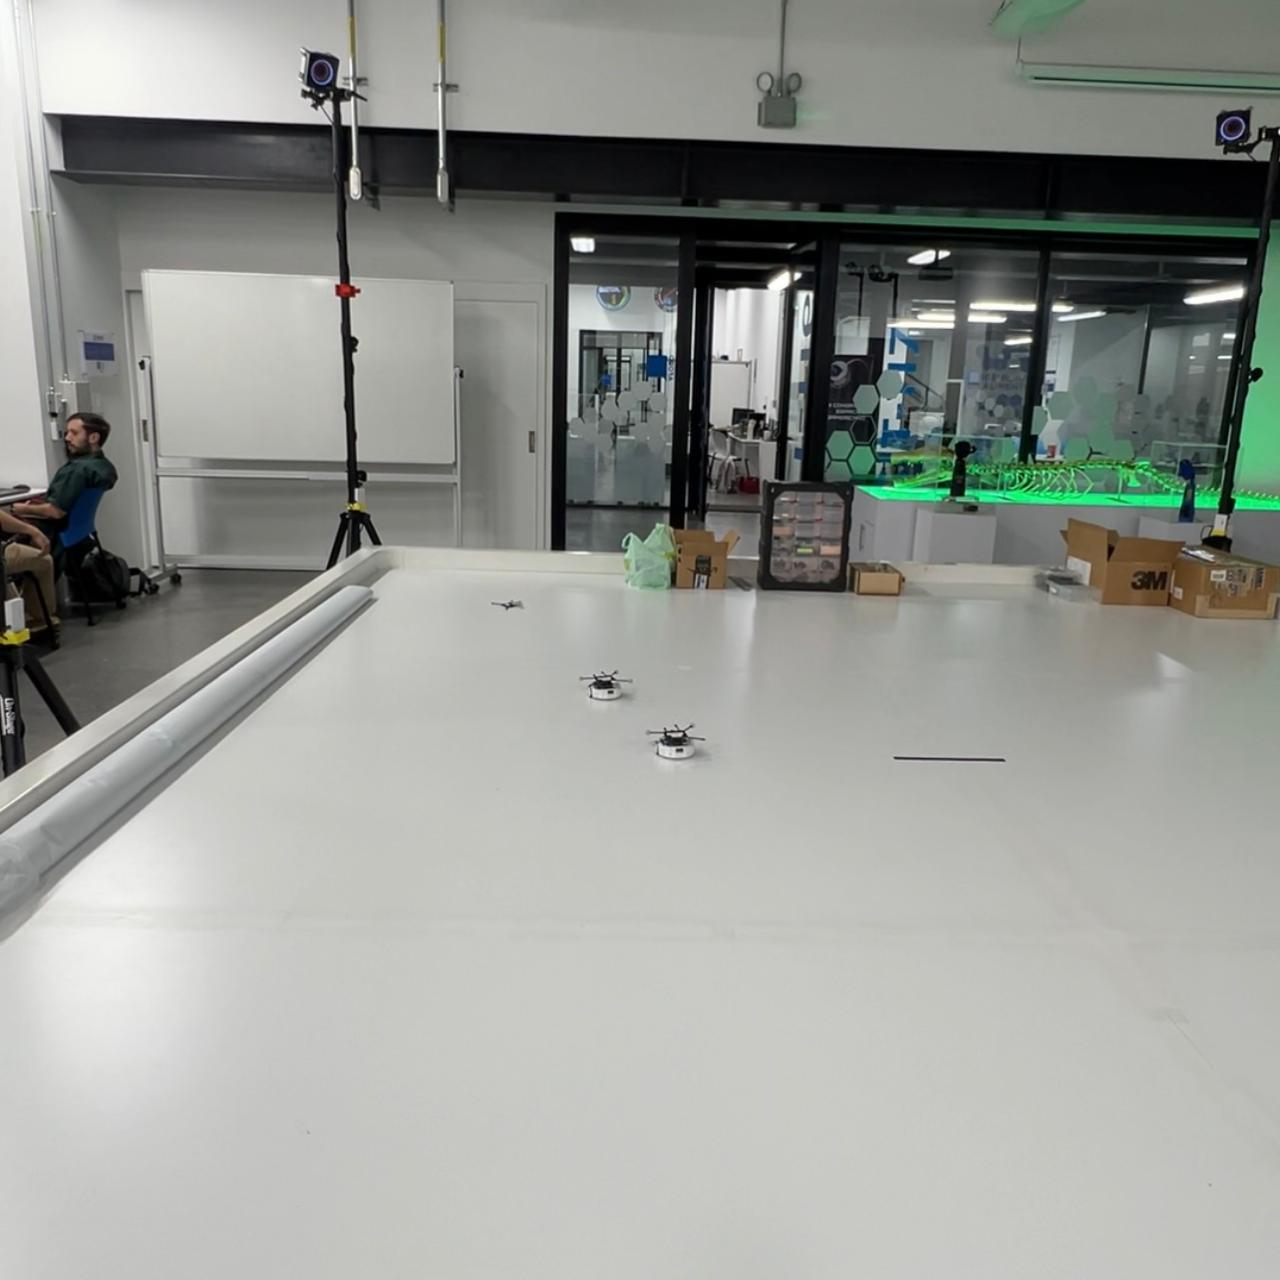
\includegraphics[width=0.45\textwidth]{prueba_fisico_p3.png}
	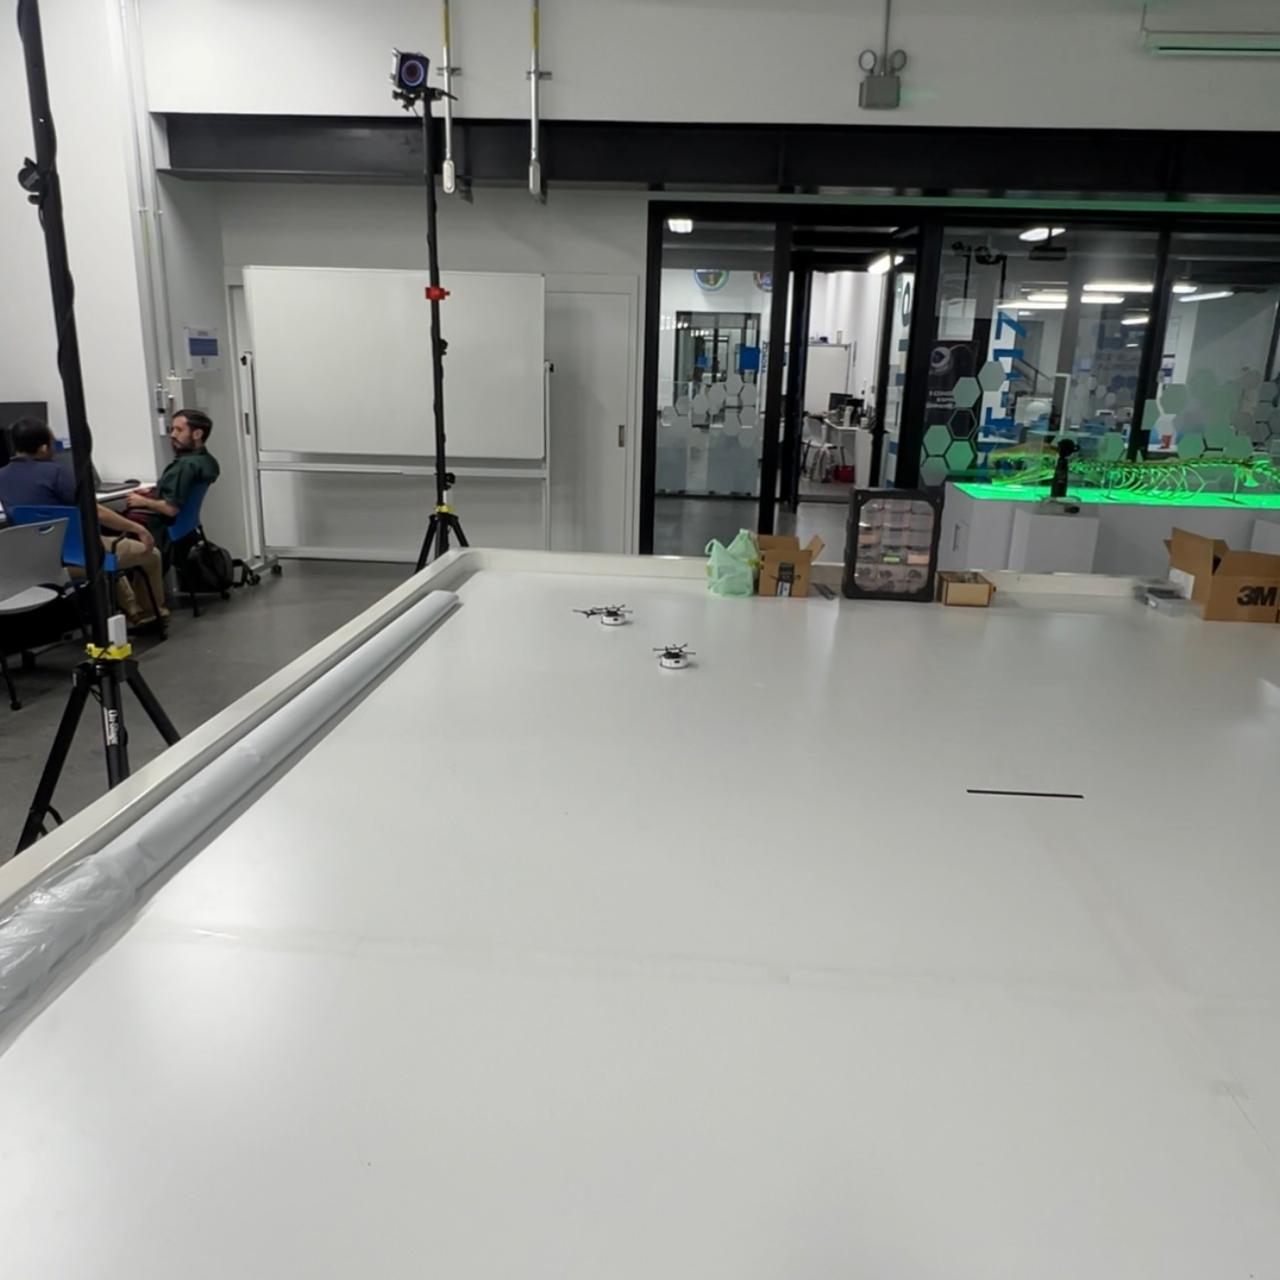
\includegraphics[width=0.45\textwidth]{prueba_fisico_p4.png}
	\caption{Primera prueba exitosa de funcionamiento en físico.}
	\label{fig:prueba_fisico1}
\end{figure}

Una vez realizada la primera prueba, se simuló un escenario arbitrario en Webots, sin embargo se encontró que ahora la simulación presentaba patrones de divergencia en todas las etapas del algoritmo. Por esto, se optó por implementar el control proporcional de la Ecuación (\ref{eq:controlador_proporcional}) para las simulaciones y otro control proporcional con la Ecuación (\ref{eq:controlador_proporcional2}) para ejecutar el algoritmo en físico.

\chapter{Optimización del algoritmo y su implementación}
En este capítulo se describen los puntos de mejora identificados en la implementación del algoritmo de sincronización y control de formaciones. Luego, se detallará cómo se abordó cada uno de ellos empleando técnicas de optimización como la reducción de complejidad computacional, ajuste de parámetros de control y paralelización de procesos.


\section{Lenguaje de programación y limpieza de código}
El primer paso para la optimización fue analizar el lenguaje de programación empleado para los controladores. Se tomó en cuenta tres lenguajes para compararlos en base a las ventajas y desventajas que proponen para su implementación con el estado actual del algoritmo: MATLAB, Python y C. En el Cuadro \ref{cuadro:lenguajes_programacion} se describen las ventajas y desventajas que tiene un lenguaje sobre otro.

\begin{table}[H]
	\centering
	\resizebox{\textwidth}{!} {
	\begin{tabular}{|l|l|l|}
		\hline
		Lenguaje & Ventajas                                                                                                                                                                                                                                                                                                     & Desventajas                                                                                                                                                                                                                                                                                                             \\ \hline
		MATLAB   & \begin{tabular}[c]{@{}l@{}}- Es fácil de usar para simulaciones y prototipos.\\ \\ - Tiene una amplia variedad de herramientas \\ matemáticas.\\ \\ - Es excelente para algoritmos que involucran \\ operaciones matriciales.\end{tabular}                                                                      & \begin{tabular}[c]{@{}l@{}}- Es un lenguaje propio de MATLAB por lo que requiere comprar \\ licencias de software.\\ \\ - Su eficiencia computacional es menor en cuanto a rendimiento \\ comparado con Python o C.\end{tabular}                                                                                          \\ \hline
		Python   & \begin{tabular}[c]{@{}l@{}}- Es un lenguaje de código abierto (\textit{open source}).\\ \\ - Tiene una amplia variedad de librerías para optimizar \\ el cálculo numérico como NumPy, SciPy, multithreading \\ o multiprocessing.\\ \\ - Tiene un buen equilibrio entre rendmiento \\ computacional y facilidad de desarrollo.\end{tabular} & \begin{tabular}[c]{@{}l@{}}- Es un lenguaje más eficiente que MATLAB pero menos eficiente \\ que C debido a que es un lenguaje interpretado.\\ \\ - Requiere dependencias externas para lograr un alto rendimiento \\ (como integraciones con C).\end{tabular}                                                            \\ \hline
		C        & \begin{tabular}[c]{@{}l@{}}- Tiene un rendimiento superior ya que es un lenguaje \\ compilado de bajo nivel.\\ \\ - Ofrece un control sobre la memoria y el hardware.\end{tabular}                                                                                                                             & \begin{tabular}[c]{@{}l@{}}- Su complejidad es mucho mayor en cuando a implementación y \\ mantenimiento.\\ \\ - Tiene una alta probabilidad de fugas de memoria. \\ \\ - Requiere mucho más tiempo de desarrollo y es menos intuitivo.\\ \\ - No es tan flexible para realizar cambios rápidos en algoritmos.\end{tabular} \\ \hline
	\end{tabular}}
	\caption{Ventajas y desventajas de lenguajes de programación.}
	\label{cuadro:lenguajes_programacion}
\end{table}

Una vez comparados los lenguajes de programación se optó por seguir utilizando Python para el desarrollo de los controladores. Las razones principales fueron que es un lenguaje de código abierto y ofrece un buen equilibrio entre rendimiento computacional y facilidad de desarrollo. Además, ya se cuenta con todo el algoritmo previo desarrollado en Python funcionando en un entorno físico como el Robotat. Esto incluye el desarrollo de los controladores, funciones para cálculos propios del algoritmo de sincronización y control de formaciones y funciones de conexión con el servidor del Robotat y los Pololu 3Pi+. Por lo que, dado el poco tiempo disponible para utilizar el Robotat no es conveniente migrar a un nuevo lenguaje de programación para esta fase de la implementación del algoritmo. Además, python cuenta con librerías como NumPy que está basada en C y otras librerías de comunicación y procesamiento que permiten optimizar el rendimiento computacional.

Finalmente, se realizó un proceso de limpieza y documentación del código para facilitar las iteraciones a realizar. Además, esto permitió eliminar segmentos de código obsoletos, así como identificar otras deficiencias que se mencionarán a continuación.

\section{Posición de cada agente según el grafo de formación}
Durante la restauración del algoritmo desarrollado en fases previas, al implementar la selección manual de marcadores para los agentes, se encontró que anteriormente el número de marcador asignado a cada agente estaba directamente relacionado con la posición que este debe tomar según el grafo de formación. En la Figura \ref{fig:grafo_formacion1} se muestra la asignación de posiciones según el grafo de formación para una selección arbitraria de agentes con la implementación original del algoritmo.

\begin{figure}[H]
	\centering
	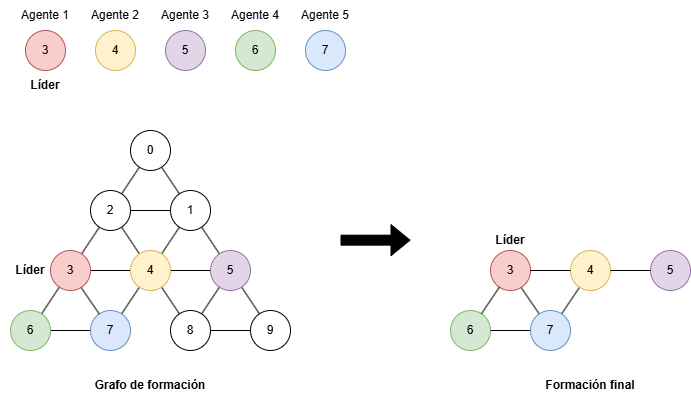
\includegraphics[width=0.8\textwidth]{grafo_formacion1.png}
	\caption{Posiciones de agentes según el grafo de formación con la implementación original del algoritmo.}
	\label{fig:grafo_formacion1}
\end{figure}

Al tener una formación como la mostrada anteriormente se vuelve poco intuitiva su visualización a la hora de ejecutar el algoritmo. Por esto, se decidió cambiar la asignación de posición de cada agente a manera que siempre se mantenga la misma estructura del grafo de formación y los agentes se posicionen de manera ascendente tal como se observa en la figura \ref{fig:grafo_formacion2}.

\begin{figure}[H]
	\centering
	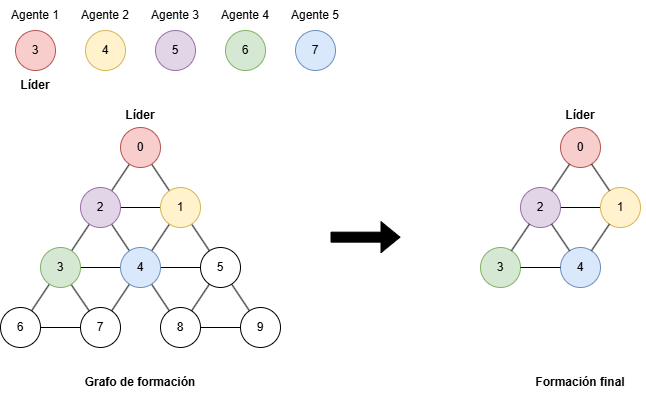
\includegraphics[width=0.8\textwidth]{grafo_formacion2.png}
	\caption{Posiciones de agentes según el grafo de formación con la implementación original del algoritmo.}
	\label{fig:grafo_formacion2}
\end{figure}
	
\section{Mejorar la eficiencia computacional con NumPy}
NumPy es una librería de Python especializada para el cálculo numérico y científico. Destaca por su soporte para trabajar con operaciones vectorizadas o vectores multidimensionales sin realizar bucles. También cuenta con una amplia variedad de funciones matemáticas y estadísticas, así como integración con otras bibliotecas como SciPy. Además, NumPy está implementado en C por lo que permite mejorar la eficiencia computacional para grandes cantidades de datos.

Al revisar los programas de los controladores, se encontró varios segmentos de código que se realizan con ciclos \textit{for} simples y otros anidados. Esto presenta una deficiencia al realizar los cálculos y solicitud de datos al servidor del Robotat por lo que se optó por optimizar dichos procesos utilizando funciones matemáticas y operaciones matriciales con NumPy. A continuación, se detallará los segmentos del algoritmo que se optimizaron implementando operaciones con NumPy y se mostrará la comparativa en cuanto a tiempos de ejecución utilizando la librería ``time'' de Python y análisis estadísticos.

\subsection{Aplicar desfases de los marcadores}
A continuación se explica los pasos que se realizaban anteriormente para aplicar los desfases de la calibración de marcadores, donde $n$ es la cantidad de marcadores a utilizar.


\begin{itemize}
	\item Configuración
	\begin{enumerate}
		\item Cargar el archivo .npy con los desfases de los marcadores.
		\item Solicitar las poses de $n$ marcadores al sevidor del Robotat.
		\item Aplicar el desfase de cada marcador con un ciclo \textit{for} de $n$ iteraciones.
	\end{enumerate}
	\item Ciclo principal 
	\begin{enumerate}
		\item Solicitar las poses de $n$ marcadores al servidor del Robotat.
		\item Aplicar el desfase de cada marcador con un ciclo \textit{for} de $n$ iteraciones.
	\end{enumerate}
\end{itemize}

Sin embargo, el implementar ciclos \textit{for} dentro del ciclo principal significa un aumento de tiempo computacional que es más notorio al aumentar la cantidad de marcadores a utilizar. Para optimizar el proceso se optó por aplicar los desfases a cada marcador utilizando operaciones matriciales e implementando únicamente una resta de matrices dentro del ciclo principal, por lo que ahora el proceso es el siguiente:

\begin{itemize}
	\item Configuración
	\begin{enumerate}
		\item Cargar el archivo .npy con los desfases de los marcadores.
		\item Almacenar los desfases en la cuarta columna de una matriz de ceros de tamaño $n \times 6$.
		\item Solicitar las poses de los marcadores al sevidor del Robotat.
		\item Aplicar el desfase de los marcadores con una resta de la matriz con los desfases a la matriz con las poses de los marcadores.
	\end{enumerate}
	\item Ciclo principal 
	\begin{enumerate}
		\item Solicitar las poses de los marcadores al servidor del Robotat
		\item Aplicar el desfase de los marcadores con una resta de la matriz con los desfases a la matriz con las poses de los marcadores.
	\end{enumerate}
\end{itemize}

Una vez implementada la optimización, se realizó un análisis estadístico con mil muestras donde se tomó el tiempo que toma aplicar los desfases a los marcadores con un ciclo \textit{for} y con una resta de matrices con NumPy.

Para la toma de muestras, se evaluó diferentes cantidades de marcadores a los que se les aplicaría el desfase, siendo estos 5, 10, 15 y 20. En los Cuadros \ref{cuadro:tiempos_desfases_for} y \ref{cuadro:tiempos_desfases_numpy} se muestra la media y desviación estándar del tiempo que toma aplicar los desfases.

En la Figura \ref{fig:grafica_tiempos_desfases} se observa que la optimización con NumPy presenta una reducción notable en el tiempo de procesamiento, la cual es aún más significativa a medida que aumenta la cantidad de marcadores a utilizar. Por otro lado, los tiempos al aplicar ciclos \textit{for} incrementan de manera proporcional y más pronunciada con el aumento de los marcadores, mientras que con NumPy el crecimiento es más moderado ya que la pendiente de la curva es dos órdenes de magnitud menor.

\begin{table}[H]
	\centering
	\resizebox{\textwidth}{!} {
	\begin{tabular}{|l|l|l|l|}
		\hline
		\textbf{Cantidad de marcadores} & \textbf{Número de muestras} & \textbf{Media de tiempo (ms)} & \textbf{Desviación estándar (ms)} \\ \hline
		5 & 1000 & 0.002802 & 0.000308 \\ \hline
		10 & 1000 & 0.005353 & 0.000469 \\ \hline
		15 & 1000 & 0.008187 & 0.001654 \\ \hline
		20 & 1000 & 0.010485 & 0.000843 \\ \hline
	\end{tabular}}
	\caption{Media de tiempo y desviación estándar para aplicar desfases de marcadores con ciclos \text{for}.}
	\label{cuadro:tiempos_desfases_for}
\end{table}

\begin{table}[H]
	\centering
	\resizebox{\textwidth}{!} {
	\begin{tabular}{|l|l|l|l|}
		\hline
		\textbf{Cantidad de marcadores} & \textbf{Número de muestras} & \textbf{Media de tiempo (ms)} & \textbf{Desviación estándar (ms)} \\ \hline
		5 & 1000 & 0.000734 & 0.000119 \\ \hline
		10 & 1000 & 0.000756 & 0.000113 \\ \hline
		15 & 1000 & 0.000794 & 0.000225 \\ \hline
		20 & 1000 & 0.000837 & 0.000147 \\ \hline
	\end{tabular}}
	\caption{Media de tiempo y desviación estándar para aplicar desfases de marcadores con NumPy.}
	\label{cuadro:tiempos_desfases_numpy}
\end{table}

\begin{figure}[H]
	\centering
	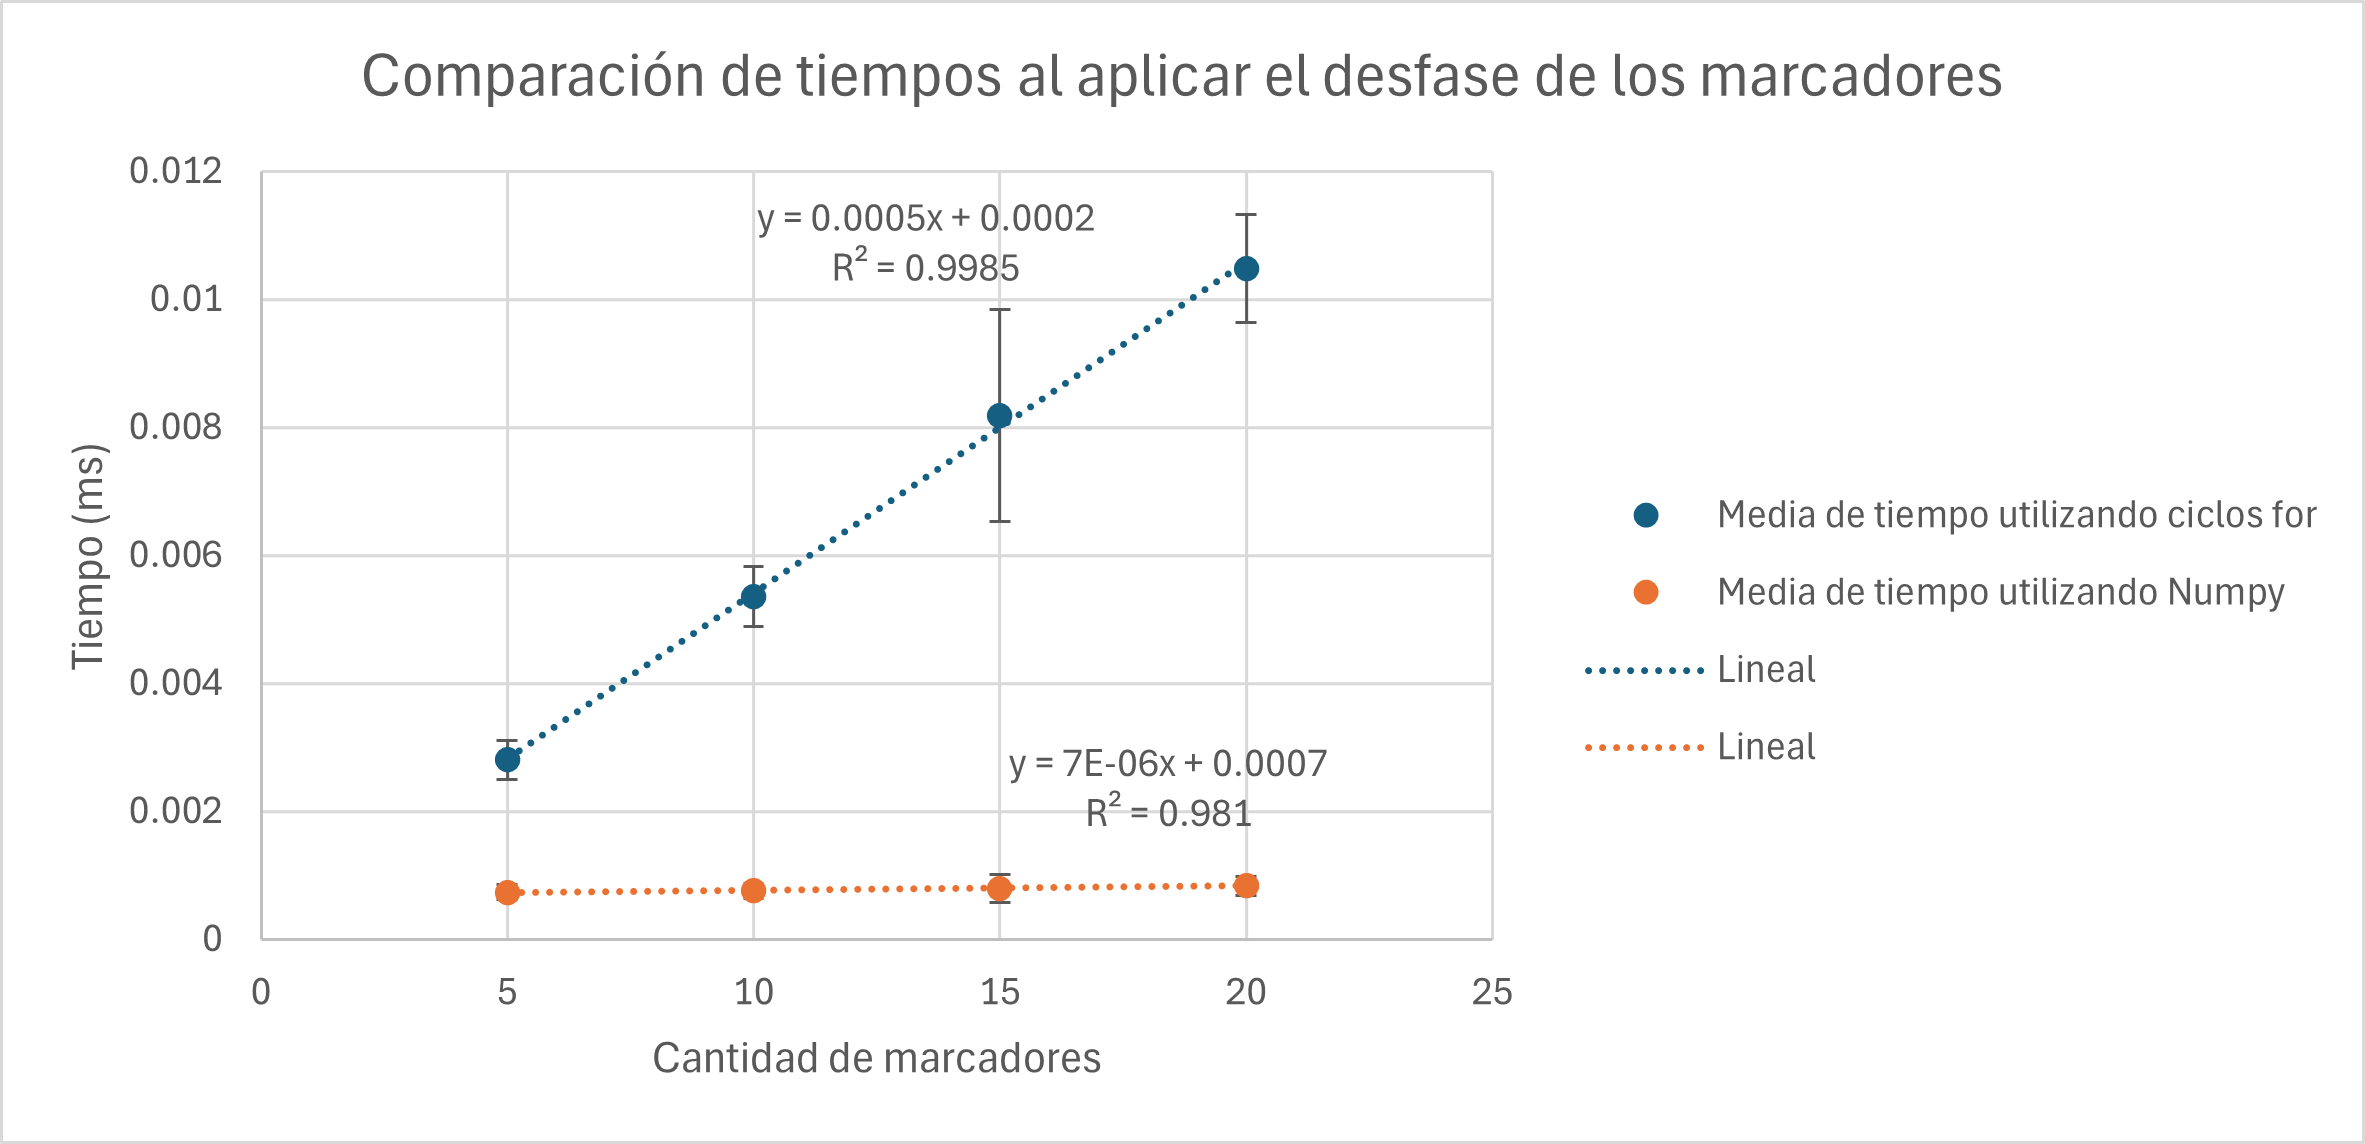
\includegraphics[width=0.8\textwidth]{tiempos_desfases.png}
	\caption{Gráfica con medias de tiempo para aplicar desfases de marcadores con ciclos \textit{for} y operaciones don NumPy.}
	\label{fig:grafica_tiempos_desfases}
\end{figure}

\subsection{Cálculo de la distancia entre agentes}
Para el cálculo de distancia entre agentes se tiene una función llamada ``DistBetweenAgents'' dentro del archivo ``funciones.py''. Esta utiliza dos ciclos \textit{for} anidados para calcular la norma de distancia basada en la distancia en $x$ y $y$ de cada agente hacia sus vecinos más próximos. El cálculo de la distancia se realiza entre los agentes $i$ y $j$ y luego para $j$ e $i$, esto produce una matriz simétrica por lo que se puede realizar únicamente el cálculo de una mitad y luego duplicarla. Para esto, se creó una versión optimizada de la función llamada ``DistBetweenAgentsOptimized''. En esta, únicamente se calcula la diferencia de posiciones aprovechando el \textit{broadcasting} en NumPy y luego calcula la norma de la matriz de distancias utilizando la función ``linealg.norm''.

En los Cuadros \ref{label} y \ref{label} se muestra la media y desviación estándar del tiempo que toma en realizar los cálculos con la función original y la optimizada.


\subsection{Cálculo del error de formación}

\section{Implementación de paralelismo computacional}





